\documentclass[11pt,twoside]{article}

\usepackage[margin=1in]{geometry}
\usepackage{amsmath,amssymb,amsthm,mathtools}
\usepackage{array,booktabs}
\usepackage[inline,shortlabels]{enumitem}
\usepackage{xcolor}
\usepackage{microtype}
\usepackage{tikz}
\usetikzlibrary{arrows.meta,positioning,calc,fit}
\usepackage{../exercises/course-exercises}

% Revision date: maintained by scripts/build_lecture_notes.py. Keep this command.
\newcommand{\lecturerevised}{2026-10-25 23:07 UTC-06:00}
\usepackage{eso-pic}
\AddToShipoutPictureBG{%
  \AtPageLowerLeft{%
    \put(\LenToUnit{0.5\paperwidth},\LenToUnit{0.5in}){%
      \makebox(0,0){\normalfont\footnotesize\color{black!60}Last revised: \lecturerevised}%
    }%
  }%
}

\usepackage[square,authoryear]{natbib}
\usepackage[colorlinks=true,linkcolor=blue!60!black,
  urlcolor=blue!60!black,citecolor=blue!60!black]{hyperref}
\newcommand{\suppmark}{\texorpdfstring{\textsuperscript{*}}{*}}
\usepackage[nameinlink,capitalize]{cleveref}
\crefname{exercise}{Exercise}{Exercises}
\Crefname{exercise}{Exercise}{Exercises}

\usepackage{enotez}
\DeclareInstance{enotez-list}{lecture}{list}{format=\normalsize,number={#1.}}
\setenotez{list-name=Endnotes,list-style=lecture,backref=true}
\crefname{endnote}{Endnote}{Endnotes}
\Crefname{endnote}{Endnote}{Endnotes}

\definecolor{courseblue}{HTML}{17365D}
\definecolor{lightblue}{HTML}{DCE6F1}
\newcommand{\E}{\mathbb E}
\newcommand{\I}{\mathbb I}
\renewcommand{\P}{\mathbb P}
\newcommand{\R}{\mathbb R}
\newcommand{\relu}{\operatorname{ReLU}}
\newcommand{\NOT}{\operatorname{NOT}}
\newcommand{\AND}{\operatorname{AND}}
\newcommand{\OR}{\operatorname{OR}}
\newcommand{\hop}{\operatorname{hop}}
\makeatletter
\@for\@letter:=A,B,C,D,E,F,G,H,I,J,K,L,M,N,O,P,Q,R,S,T,U,V,W,X,Y,Z\do{%
  \expandafter\edef\csname c\@letter\endcsname{\noexpand\mathcal{\@letter}}}
\makeatother
\newcommand{\lecturenumber}{14}

\newtheorem{theorem}{Theorem}[section]
\newtheorem{proposition}[theorem]{Proposition}
\newtheorem{corollary}[theorem]{Corollary}
\newtheorem{lemma}[theorem]{Lemma}
\theoremstyle{definition}
\newtheorem{definition}[theorem]{Definition}
\newtheorem{example}[theorem]{Example}
\theoremstyle{remark}
\newtheorem{remark}[theorem]{Remark}

\renewcommand{\thepage}{14--\arabic{page}}
\renewcommand{\thesection}{14.\arabic{section}}
\renewcommand{\theequation}{14.\arabic{equation}}
\pagestyle{myheadings}
\markboth{Lecture 14: Neural networks as computational models}
{Lecture 14: Neural networks as computational models}

\begin{document}

\begin{center}
\fcolorbox{courseblue}{white}{%
\begin{minipage}{0.92\textwidth}
\vspace{1mm}
\textbf{CMPUT 654: Mathematical Foundations of Modern AI Systems}
\hfill Fall 2026

\vspace{3mm}
\begin{center}
{\Large\bfseries Lecture 14: Neural networks as computational models}

\vspace{1mm}
October 20, 2026
\end{center}

\vspace{2mm}
\textit{Lecturer: Csaba Szepesv\'ari}
\hfill
\textit{Note prepared by: Csaba Szepesv\'ari}
\vspace{1mm}
\end{minipage}}
\end{center}

\noindent\textbf{Reading guide.}
Lecture 13 asked what a learned representation preserves for later tasks.
This lecture asks whether neural networks can represent symbolic computation.
With repeated application and an external memory, the answer is yes. The
Church--Turing thesis reduces the question to simulating a Turing machine, and
a Turing machine separates into a finite controller and an unbounded tape. A
neural network therefore needs to implement only a finite transition table.
Bit encodings turn the table into Boolean functions, and Boolean circuits
compile exactly into ReLU networks.

The remaining topics study how computational resources and the location of a
map affect how the map is represented. A repeated tent-map construction shows
that
depth can make an exact representation exponentially smaller. Associative and
iterated lookup move the map from the network parameters into the input and
ask how a sequence model can apply and compose the supplied map.

The material presented in class runs through \cref{sec:routing}.
The starred Boolean-depth section is supplementary. Section~14.4 and all
later sections are extra reading; they separate program correctness from
learning, record arithmetic assumptions, and give a conditional lower bound.
The main arguments require only elementary finite mathematics, algebra, and
induction.

The exact constructions establish representability and resource counts. They
do not show that training will find the required computation. The extra
reading in \cref{sec:claims} returns to the learning question. Lecture 15
replaces exact equality by approximation error and studies the resulting
tradeoff.

\section{From symbolic computation to Boolean circuits}
\label{sec:gates}

\subsection{What symbolic computation meant}

The physical symbol system hypothesis proposed that general intelligent
action requires and can be produced by a system that stores symbol structures
and transforms them by explicit rules. Here a symbol structure is a
well-formed expression in a formal language. To specify the syntax of a formal
language, one starts with primitive symbols and formation rules that determine
which finite strings are well formed. In first-order logic, the nonlogical
vocabulary contains constant, function, and relation symbols; variables,
logical connectives, and quantifiers are also part of the syntax. A memory can
store one well-formed sentence or a collection of sentences. Explicit
inference or rewrite rules transform stored expressions into other
well-formed expressions. Classical symbolic AI used formal expressions and
explicit transformation rules to represent knowledge and carry out deductions.

The symbol grounding problem asks how the formal symbols in such a system
become connected to objects, properties, and situations outside the formal
system. Syntactic rules determine how one expression produces another, but
syntax alone does not determine that a particular constant refers to a
particular person or object. An external user can supply an interpretation.
The grounding problem asks how the system itself can acquire and maintain the
connections expressed by such an interpretation.

Machine learning eliminates the requirement that a designer enumerate a
complete symbolic knowledge base and every rule for manipulating the stored
expressions. A learning algorithm instead receives data from outside the
formal system and uses the observations and feedback to shape the system's
behavior. For a dialogue system, the data can include utterances, responses,
and feedback. For a robot, the data
can include sensor observations, actions, and their consequences. The
relation to the external world can therefore enter through data and
interaction rather than only through a hand-written interpretation.

Sequence models add the ability to learn transformations whose inputs and
outputs are strings. Well-formed expressions of a formal language are strings,
so a learned sequence model can carry out syntactic symbol manipulation as
part of the model's behavior. Machine learning therefore bypasses the
requirement that all knowledge and manipulation rules be written down in
advance. Learning string transformations does not guarantee exact,
systematic, or reliable symbol manipulation.

Neural networks are not excluded from symbolic computation by their
mathematical form. Recurrent neural networks, and neural networks combined
with external memory, were known to simulate universal computation before the
development of modern sequence models. The remaining question is whether
data, objectives, and optimization produce the required computation reliably.
Current systems can perform broadly and still fail on closely related inputs,
so the learning question remains open. Current systems also use scratchpads,
retrieval, tools, and other external memory. The division used in the
Turing-machine construction below therefore reappears: a learned finite
component operates together with a memory environment. Lecture~16 studies the
resources supplied by the memory environment.

\subsection{Turing machines reduce universality to finite control}

The Church--Turing thesis identifies effectively calculable procedures with
the functions computable by a Turing machine. The thesis is not a theorem
about an independently formalized notion of every possible procedure; the
thesis states the intended scope of the formal model. A deterministic Turing
machine
has a finite state set $Q$, a finite tape alphabet $\Gamma$, a head that reads
and writes one tape cell, and an unbounded tape. One step applies a finite
transition function
\begin{equation}
 \delta:Q\times\Gamma
 \longrightarrow Q\times\Gamma\times\{\mathtt L,\mathtt R\}.
 \label{eq:turing-transition}
\end{equation}
The output specifies the next state, the symbol written at the current cell,
and the head movement. The tape and head are the memory environment; the
transition function is the finite controller.

Suppose a neural network computes an exact bit encoding of $\delta$. Reapply
the same network after every tape update. Induction over time shows that the
network-controlled system has exactly the same state, tape, and head position
as the Turing machine after every step. A universal Turing machine has one
fixed transition function and receives the simulated machine description and
input on the tape. Consequently, universal computation requires the neural component
to represent only one fixed finite table, provided that the environment
supplies an unbounded read--write tape and permits repeated application. A
fixed feedforward network without an external tape and repeated execution does
not by itself perform an arbitrarily long computation.

\subsection{Finite transition tables are Boolean functions}

Encode the state, scanned symbol, next state, written symbol, and head
direction by bits. After extending the transition rule arbitrarily on unused
bit strings, each output bit is a Boolean function
\[
 f:\{0,1\}^r\longrightarrow\{0,1\}.
\]
There are $2^{2^r}$ such functions: a truth table contains $2^r$ rows, and
each row receives one of two output bits. A transition rule with $s$ output
bits therefore has $(2^{2^r})^s=2^{s2^r}$ possible truth tables.

Circuits represent a many-input Boolean function by composing gates with
smaller fan-in. Unary gates are insufficient: the four unary Boolean
functions are the two constants, the identity, and negation, and a circuit
made only of unary gates cannot combine two input coordinates.
\Cref{ex:l14-boolean-circuit} asks for the proof. There are sixteen binary
Boolean functions, including constants, projections and their negations,
$\AND$, $\OR$, NAND, NOR, XOR, and the remaining binary gates.
The goal is to find a small collection of gates from which every finite truth
table can be built.

Boolean circuits also record two resources that the later compilation should
preserve: size measures the number of gates, while depth measures the number
of sequential stages. A circuit-to-ReLU translation can therefore establish
representability and compare resources.

Write
\[
 \relu(t)=\max\{0,t\}.
\]
On bit inputs $x,y\in\{0,1\}$, the formulas
\begin{equation}
 \NOT(x)=1-x,
 \qquad
 \AND(x,y)=\relu(x+y-1)
 \label{eq:not-and}
\end{equation}
are exact. The truth table for $\AND$ follows because $x+y-1$ is positive
only when $x=y=1$. De Morgan's law then gives
\begin{equation}
 \OR(x,y)=\NOT\bigl(\AND(\NOT(x),\NOT(y))\bigr).
 \label{eq:or-by-composition}
\end{equation}
The De Morgan construction makes circuit composition explicit: once a network
implements a collection of gates, connecting the gate outputs builds a larger
computation. A more compact formula for $\OR$ is recorded in an
endnote.\endnote{For $x,y\in\{0,1\}$,
$\OR(x,y)=x+y-\relu(x+y-1)$. The De Morgan construction in
\cref{eq:or-by-composition} exposes circuit composition more directly.}

\begin{figure}[ht]
\centering
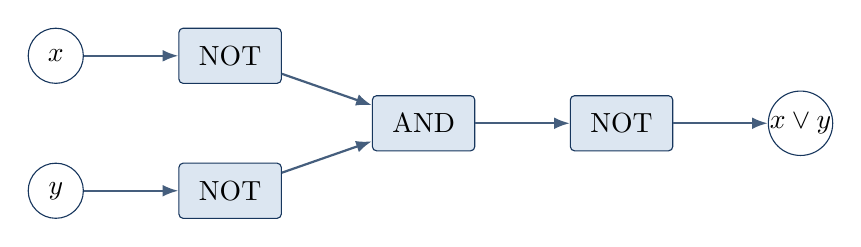
\begin{tikzpicture}[
  bit/.style={circle,draw=courseblue,minimum size=7mm,inner sep=0pt},
  gate/.style={draw=courseblue,fill=lightblue,rounded corners=1.5pt,
    minimum width=13mm,minimum height=7mm},
  arr/.style={-{Latex[length=2mm]},thick,courseblue!80},
  node distance=9mm and 12mm]
  \node[bit] (x) {$x$};
  \node[bit,below=10mm of x] (y) {$y$};
  \node[gate,right=of x] (nx) {NOT};
  \node[gate,right=of y] (ny) {NOT};
  \node[gate,right=18mm of $(nx)!0.5!(ny)$] (a) {AND};
  \node[gate,right=of a] (o) {NOT};
  \node[bit,right=of o] (z) {$x\lor y$};
  \draw[arr] (x)--(nx); \draw[arr] (y)--(ny);
  \draw[arr] (nx)--(a); \draw[arr] (ny)--(a);
  \draw[arr] (a)--(o); \draw[arr] (o)--(z);
\end{tikzpicture}
\caption{The ReLU realization of OR obtained by composing NOT and AND. The
diagram is also a small circuit-compilation example.}
\label{fig:or-composition}
\end{figure}

\begin{definition}[Boolean circuit]
A Boolean circuit is a finite directed acyclic graph. Source nodes contain
input bits. Every non-source node applies one of $\NOT$, $\AND$, and $\OR$ to
the values at its incoming edges. The \emph{size} is the number of gates, and
the \emph{depth} is the maximum number of gates on an input-to-output path.
\end{definition}

The literature allows many choices of primitive gates. A set of Boolean
gates is \emph{functionally complete}, or \emph{universal}, if circuits using
those gates compute every Boolean function on every finite number of inputs.
Among subsets of $\{\AND,\OR,\NOT\}$, a set is universal exactly when it
contains $\NOT$ and at least one of $\AND$ and $\OR$. Sufficiency follows
from De Morgan's laws. For necessity, circuits without $\NOT$ compute only
monotone functions, while circuits made only from $\NOT$ cannot combine two
input bits. No one gate in the displayed three-gate set is individually
necessary: NAND alone is universal because
\[
 \NOT(x)=\operatorname{NAND}(x,x),
 \qquad
 \AND(x,y)=\NOT(\operatorname{NAND}(x,y)).
\]
The analogous statement holds for NOR.

Functional completeness is what makes circuits a general representation
tool, rather than a collection of examples. Once a finite input and output
are encoded by bits, the desired computation is a Boolean function. The next
theorem constructs a circuit for every such function.

\begin{theorem}[Every Boolean function has a circuit]
\label{thm:boolean-universality}
For every integer $n\geq1$ and every function
$f:\{0,1\}^n\to\{0,1\}$, there is an $\{\AND,\OR,\NOT\}$ circuit that
computes $f$.
\end{theorem}

\begin{proof}
For each $a\in\{0,1\}$, $x\in \{0,1\}$, define the literal
\[
 \ell_{a}(x)=
 \begin{cases}
  x,&a=1,\\
  \NOT(x),&a=0,
 \end{cases}
 \]
and for $a,x\in \{0,1\}^n$, let
\[
 m_a(x)=\bigwedge_{i=1}^n\ell_{a_i}(x_i).
\]
The conjunction $m_a(x)$ equals one exactly when $x=a$. Therefore
\begin{equation}
 f(x)=\bigvee_{\substack{a\in\{0,1\}^n\\ f(a)=1}}m_a(x).
 \label{eq:dnf}
\end{equation}
If the index set in \cref{eq:dnf} is empty, use
$x_1\land\NOT(x_1)$ for the constant-zero function. Binary trees of gates
implement the displayed finite conjunctions and disjunction.
\end{proof}

The explicit construction uses at most $O(n2^n)$ gates. The theorem proves
universality, not economy. Circuit complexity asks whether a particular
function has a much smaller circuit.

\begin{theorem}[Exact simulation of Boolean circuits]
\label{thm:circuit-simulation}
Let $C$ be a Boolean circuit with bounded fan-in, size $S$, and depth $D$.
There is a ReLU network that agrees with $C$ on every Boolean input, uses
$O(S)$ ReLU units, and has depth $O(D)$.
\end{theorem}

\begin{proof}
Order the circuit gates by circuit layer. Replace every gate by the
constant-size ReLU gadget in \cref{eq:not-and,eq:or-by-composition}. When an
edge must cross an added network layer, transmit its bit using
$\relu(z)=z$ for $z\in\{0,1\}$.

The correctness proof is induction over circuit layers. The input layer
agrees by construction. Suppose every wire entering circuit layer $d$
carries the same bit in the circuit and in the ReLU network. Each replacement
gadget computes the corresponding gate exactly on the incoming bits, so every wire
leaving layer $d$ also agrees. The induction proves equality at the output.
Every circuit gate contributes only a constant number of ReLU units and
network layers, which gives the stated resource bounds.
\end{proof}

Combining \cref{thm:boolean-universality,thm:circuit-simulation} shows that
ReLU networks represent every Boolean function exactly. More strongly, when
a Boolean function has a circuit of size $S$ and depth $D$, the compiled
ReLU network preserves size and depth up to constant factors.

\begin{corollary}[Neural finite control with an external tape]
\label{cor:neural-turing-control}
For every deterministic Turing machine with finite state set and finite tape
alphabet, a finite ReLU network can implement its transition function exactly
on valid bit encodings. Repeatedly applying that network while the environment
updates the tape and head simulates the Turing machine step for step. In
particular, one fixed finite ReLU controller coupled to an unbounded tape can
simulate a universal Turing machine.
\end{corollary}

\begin{proof}
Each output bit of the finite transition table in
\cref{eq:turing-transition} is a Boolean function of the encoded current
state and scanned symbol. Apply
\cref{thm:boolean-universality,thm:circuit-simulation} to each output bit,
sharing subcircuits if desired. The resulting network produces the encoded
next state, written symbol, and head direction exactly. Induction over the
number of steps proves equality with the Turing-machine execution. Choosing a
universal Turing machine makes the finite controller independent of the
simulated program. The simulated program is supplied on the tape.
\end{proof}

The corollary settles an existence question under an explicit environment.
The corollary does not bound the resources needed for a useful algorithm or
show that a training procedure finds the controller. The rest of the lecture
studies representation size and computations whose data arrive in the input.

\section{Why depth can be exponentially more economical}
\label{sec:tent}

Does depth reduce the number of ReLU units needed to represent a function?
We will prove that it can. For every $L$, we will construct a function that a
depth-$O(L)$ ReLU network represents with $O(L)$ units, while every exact
one-hidden-layer representation of the same function requires at least
$2^L-1$ units. Allowing depth therefore reduces the required size from
exponential in $L$ to linear in $L$ for this family.

We first name the network classes used in the comparison. For integers
$L,m\geq1$, let $\cF_{L\text{-NN}}(m)$ be the class of functions
$f:\R\to\R$ represented by a ReLU network with $L$ hidden layers and at most
$m$ hidden ReLU units in total. Each hidden layer applies an affine map and
coordinatewise ReLU, and the output layer is affine. Write
\[
 \cF_{L\text{-NN}}=\bigcup_{m\geq1}\cF_{L\text{-NN}}(m).
\]
For scalar functions, network composition gives
\begin{equation}
 f\in\cF_{L\text{-NN}}(m),\quad
 g\in\cF_{K\text{-NN}}(n)
 \quad\Longrightarrow\quad
 f\circ g\in\cF_{(L+K)\text{-NN}}(m+n).
 \label{eq:nn-class-composition}
\end{equation}
The class notation separates the depth of a representation from the
particular parameter values used to obtain the representation.

The proof needs a property of a function that grows exponentially when small
networks are composed but grows only linearly with the width of one hidden
layer. For scalar piecewise-affine functions, the number of affine pieces has
exactly these two features. Each scalar ReLU in one hidden layer introduces
at most one new breakpoint, so $m$ hidden units produce at most $m+1$ affine
pieces. Repeated composition can split every existing affine piece at once.

The tent map makes both sides of the comparison explicit. The map has two
affine pieces, and a constant-size ReLU module computes the tent map exactly.
Every
piece maps its half of the domain onto all of $[0,1]$, so one more composition
splits every current piece into two. Stacking $L$ copies of the module gives a
deep network with $O(L)$ units and $2^L$ affine pieces. A one-hidden-layer
network must create the corresponding $2^L-1$ breakpoints one at a time. The
rest of the section proves these two statements.

The tent map is the continuous piecewise-affine function
\begin{equation}
 \tau(x)=\min\{2x,2-2x\}
 =\begin{cases}
   2x,&0\leq x\leq\tfrac12,\\
   2-2x,&\tfrac12\leq x\leq1
  \end{cases}
 \qquad (x\in[0,1]).
 \label{eq:tent-definition}
\end{equation}
The graph joins $(0,0)$, $(1/2,1)$, and $(1,0)$. The slope of $\tau$ starts at
$2$ and changes by $-4$ at $1/2$. Because $\relu(x-1/2)$ introduces exactly
the slope change at $1/2$,
\[
 \tau(x)=2x-4\relu\left(x-\frac12\right),
 \qquad x\in[0,1].
\]
Extending the tent map by zero outside $[0,1]$ gives the global ReLU formula
\begin{equation}
 \tau(x)=2\relu(x)-4\relu\left(x-\frac12\right)
          +2\relu(x-1),
 \qquad x\in\R.
 \label{eq:tent}
\end{equation}
Thus one hidden ReLU layer followed by an affine readout represents the tent
map exactly: $\tau\in\cF_{1\text{-NN}}(3)$. A network with one hidden ReLU
layer and an affine output layer is also called a two-layer ReLU network when
both affine maps are counted as layers.

Values of the zero extension outside $[0,1]$ do not affect iterations starting
in $[0,1]$ because $\tau([0,1])=[0,1]$. The extension makes
$\tau$ a standard network function $\R\to\R$ represented without a direct
linear skip from input to output, so copies of the same module can be
composed using \cref{eq:nn-class-composition}. The graph is also called a
\emph{triangle function} in the neural-network depth literature. A periodic
extension would be a triangle wave; no periodic extension is used here.

The tent map and its iterates are classical objects in one-dimensional
dynamical systems.\endnote{\textbf{The tent map in dynamical systems.}
The full-height tent map is an exactly solvable model used to study symbolic
dynamics, periodic orbits, invariant measures, mixing, sensitivity to initial
conditions, and entropy. Recording whether each iterate lies to the left or
right of $1/2$ gives binary symbolic dynamics, apart from the usual ambiguity
at points whose orbit reaches $1/2$. The $2^L$ affine pieces of
$\tau^{\circ L}$ imply topological entropy $\log 2$. The orbit
$2/9\mapsto4/9\mapsto8/9\mapsto2/9$ has least period three, so the
Li--Yorke theorem applies \citep{li1975}. The commonly pictured logistic map
$f(x)=4x(1-x)$ is not merely similar: the logistic map is topologically
conjugate to the tent map through $h(x)=\sin^2(\pi x/2)$, since
$f\circ h=h\circ\tau$. See \citet{alligood1997} for the surrounding
dynamical-systems theory.}
The neural-network construction uses one further observation: a small ReLU
module computes the classical map exactly. Reusing that module by composition
produces the $L$-fold map $\tau^{\circ L}$.

\begin{figure}[ht]
\centering
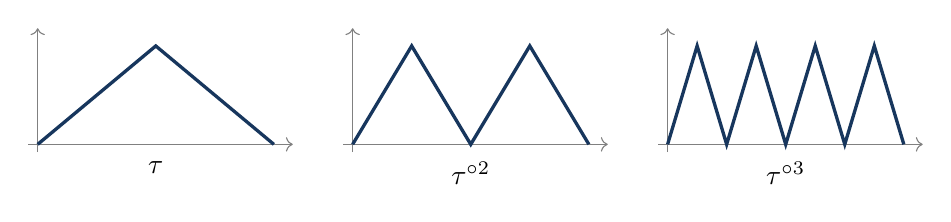
\begin{tikzpicture}[x=3.0cm,y=1.25cm]
  \begin{scope}
    \draw[->,gray] (-.04,0)--(1.08,0);
    \draw[->,gray] (0,-.08)--(0,1.18);
    \draw[very thick,courseblue] plot coordinates {(0,0) (.5,1) (1,0)};
    \node[below] at (.5,-.08) {$\tau$};
  \end{scope}
  \begin{scope}[xshift=4.0cm]
    \draw[->,gray] (-.04,0)--(1.08,0);
    \draw[->,gray] (0,-.08)--(0,1.18);
    \draw[very thick,courseblue] plot coordinates
      {(0,0) (.25,1) (.5,0) (.75,1) (1,0)};
    \node[below] at (.5,-.08) {$\tau^{\circ2}$};
  \end{scope}
  \begin{scope}[xshift=8.0cm]
    \draw[->,gray] (-.04,0)--(1.08,0);
    \draw[->,gray] (0,-.08)--(0,1.18);
    \draw[very thick,courseblue] plot coordinates
      {(0,0) (.125,1) (.25,0) (.375,1) (.5,0)
       (.625,1) (.75,0) (.875,1) (1,0)};
    \node[below] at (.5,-.08) {$\tau^{\circ3}$};
  \end{scope}
\end{tikzpicture}
\caption{Each composition folds every existing affine piece into two pieces.
The visible counts are $2$, $4$, and $8$.}
\label{fig:tent-iterates}
\end{figure}

The standard \emph{cobweb diagram} for a dynamical system makes the
composition rule visible in a different way. Start at $x_0$ on the horizontal
axis, move vertically to the graph of $\tau$, move horizontally to the line
$y=x$, and repeat. The successive diagonal coordinates are
$x_1=\tau(x_0),x_2=\tau(x_1),\ldots$.

\begin{figure}[ht]
\centering
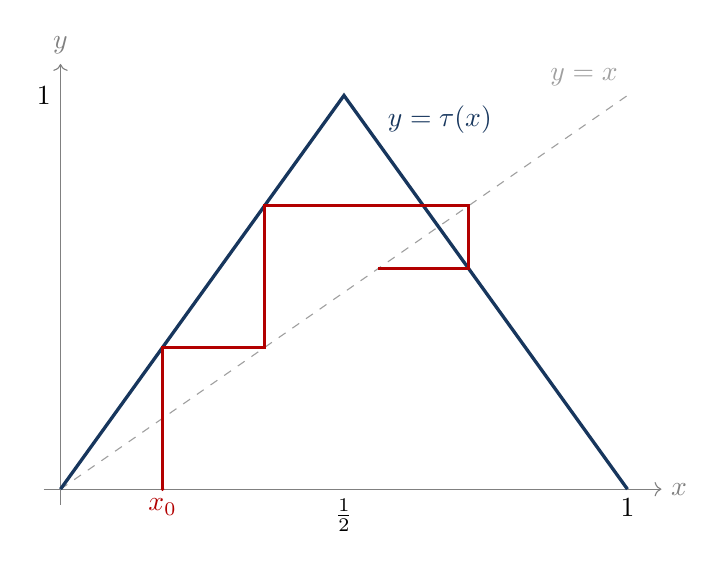
\begin{tikzpicture}[x=7.2cm,y=5.0cm]
  \draw[->,gray] (-.03,0)--(1.06,0) node[right] {$x$};
  \draw[->,gray] (0,-.04)--(0,1.08) node[above] {$y$};
  \draw[gray!75,dashed] (0,0)--(1,1) node[above left] {$y=x$};
  \draw[very thick,courseblue] plot coordinates {(0,0) (.5,1) (1,0)};
  \node[courseblue,above right] at (.56,.88) {$y=\tau(x)$};
  \draw[very thick,red!70!black]
    (.18,0)--(.18,.36)--(.36,.36)--(.36,.72)--(.72,.72)--
    (.72,.56)--(.56,.56);
  \fill[red!70!black] (.18,0) circle (.7pt);
  \node[below,red!70!black] at (.18,0) {$x_0$};
  \node[below] at (.5,0) {$\tfrac12$};
  \node[below] at (1,0) {$1$};
  \node[left] at (0,1) {$1$};
\end{tikzpicture}
\caption{A cobweb diagram for the tent map. Alternating vertical moves to
the graph and horizontal moves to the diagonal displays repeated application
of the same map.}
\label{fig:tent-cobweb}
\end{figure}

\begin{proposition}[Repeated folding]
\label{prop:tent-pieces}
For every integer $L\geq1$, the function $\tau^{\circ L}$ has exactly $2^L$
maximal affine pieces on $[0,1]$. More precisely, $\tau^{\circ L}$ is affine on every
dyadic interval
\[
 I_{L,j}=\left[\frac{j}{2^L},\frac{j+1}{2^L}\right],
 \qquad j=0,\ldots,2^L-1,
\]
and $\tau^{\circ L}$ maps each interval onto $[0,1]$.
\end{proposition}

\begin{proof}
The proposition holds for $L=1$ because the two halves of $[0,1]$ are mapped
affinely onto $[0,1]$. Suppose the proposition holds at depth $L$. On each
interval
$I_{L,j}$, the function $\tau^{\circ L}$ is affine and covers $[0,1]$.
Consequently, there is one point in the interior of $I_{L,j}$ at which
$\tau^{\circ L}(x)=1/2$. Composing with $\tau$ folds the graph at the preimage
of $1/2$ and splits $I_{L,j}$ into two affine pieces, each of which maps onto
$[0,1]$. The split points are the dyadic points at resolution $2^{-(L+1)}$.
Induction gives $2^{L+1}$ pieces at the next depth.
\end{proof}

Equation~\eqref{eq:tent} uses three ReLU units. Applying the same three-unit
module $L$ times therefore realizes $\tau^{\circ L}$ with depth $L$, width
three, and $O(L)$ units. The next proposition gives the number of units needed
by a single hidden layer to represent the same function.

\begin{proposition}[Breakpoint count for one hidden layer]
\label{prop:shallow-pieces}
Let
\begin{equation}
 f(x)=a_0+a_1x+\sum_{r=1}^m c_r\relu(w_rx+b_r).
 \label{eq:shallow-relu}
\end{equation}
The function $f$ has at most $m+1$ affine pieces on the real line. Hence an
exact representation of $\tau^{\circ L}$ in the form
\eqref{eq:shallow-relu} requires $m\geq2^L-1$.
\end{proposition}

\begin{proof}
If $w_r\neq0$, the $r$th ReLU term has one possible breakpoint,
$-b_r/w_r$. A term with $w_r=0$ has no breakpoint. After ordering the at most
$m$ distinct breakpoints, every summand and therefore their sum is affine on
each of the at most $m+1$ intervening intervals. Proposition
\ref{prop:tent-pieces} gives $2^L$ maximal affine pieces for
$\tau^{\circ L}$, so $m+1\geq2^L$ is necessary.
\end{proof}

\begin{theorem}[Folding depth separation]
\label{thm:folding-depth-separation}
For every integer $L\geq1$,
\[
 \tau^{\circ L}\in\cF_{L\text{-NN}}(3L),
 \qquad
 \tau^{\circ L}\notin\cF_{1\text{-NN}}(2^L-2).
\]
The lower bound remains valid for the larger shallow class that also
allows an affine skip $a_0+a_1x$ in the output.
\end{theorem}

\begin{proof}
The three-unit representation in \cref{eq:tent} and the composition rule
\eqref{eq:nn-class-composition} give the first membership. Every function in
$\cF_{1\text{-NN}}(m)$ has the form \eqref{eq:shallow-relu} with $a_1=0$.
\Cref{prop:shallow-pieces} shows that equality with $\tau^{\circ L}$ requires
$m\geq2^L-1$, even when an affine skip is allowed.
\end{proof}

The theorem is an exact representation statement for one function family.
Composition reuses the same small folding operation; a single hidden layer
must list all breakpoints separately.

\section*{Optional: depth separation on Boolean inputs}

The tent-map argument raises a natural question. Does the binary branching
of the dyadic intervals conceal a depth separation for Boolean functions?
The answer is partly yes. The $2^L$ intervals form a binary tree whose leaves
have addresses in $\{0,1\}^L$. The tent-map construction does not, however,
use the adjacency structure of the $L$-dimensional hypercube. More
importantly, the scalar lower bound can disappear when the interval address
is presented as bits rather than as one high-precision real number.

\begin{figure}[ht]
\centering
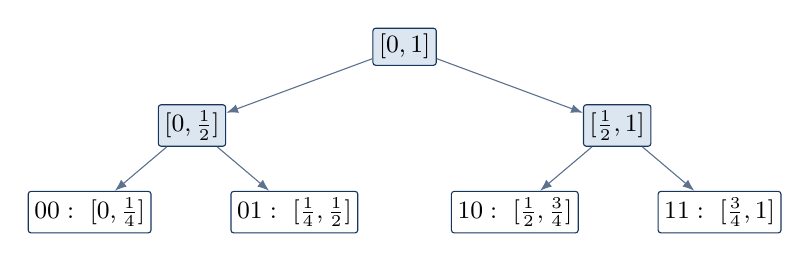
\begin{tikzpicture}[
  inode/.style={draw=courseblue,rounded corners=1pt,fill=lightblue,
    inner sep=2.2pt,font=\small},
  leaf/.style={draw=courseblue,rounded corners=1pt,inner sep=2.2pt,
    font=\small},
  edge from parent/.style={draw=courseblue!70,-{Latex[length=1.5mm]}},
  level 1/.style={sibling distance=5.4cm,level distance=10mm},
  level 2/.style={sibling distance=2.6cm,level distance=11mm}]
  \node[inode] {$[0,1]$}
    child {node[inode] {$[0,\tfrac12]$}
      child {node[leaf] {$00:\ [0,\tfrac14]$}}
      child {node[leaf] {$01:\ [\tfrac14,\tfrac12]$}}}
    child {node[inode] {$[\tfrac12,1]$}
      child {node[leaf] {$10:\ [\tfrac12,\tfrac34]$}}
      child {node[leaf] {$11:\ [\tfrac34,1]$}}};
\end{tikzpicture}
\caption{The dyadic intervals form a binary tree. At depth $L$, an
$L$-bit address identifies one of $2^L$ leaves. The tree structure alone
does not make the leaves into the Boolean hypercube graph.}
\label{fig:dyadic-tree}
\end{figure}

The next proposition makes the role of the input encoding precise.

\begin{proposition}[One table under two encodings]
\label{prop:tent-boolean-grid}
Let $N=2^L$, $x_j=j/N$, and
$y_j=\tau^{\circ L}(x_j)$ for $j=0,\ldots,N-1$. Then
$y_j=j\bmod 2$. If a one-hidden-layer scalar ReLU network of the form
\eqref{eq:shallow-relu} satisfies $f(x_j)=y_j$ at all $N$ points, then
$m\geq N/2-1$. In contrast, if $j$ is presented by its $L$-bit binary
expansion $b_1\cdots b_L$, with $b_L$ the least significant bit, then the
same table is computed by the coordinate projection $b\mapsto b_L$.
\end{proposition}

\begin{proof}
The identity
\[
 \tau^{\circ L}(x)=2\,\operatorname{dist}
       \bigl(2^{L-1}x,\mathbb Z\bigr),\qquad x\in[0,1],
\]
gives the alternating values on the dyadic grid. For the lower bound, take
second differences across consecutive grid points. The target sequence has
$y_{j+1}-2y_j+y_{j-1}\neq0$ for every $j=1,\ldots,N-2$. The affine part of
\eqref{eq:shallow-relu} has zero second difference, and the sampled values of
one ReLU hinge have nonzero second differences at at most two adjacent
indices. Consequently, $2m\geq N-2$, so at least $N/2-1$ hinges are
necessary. The coordinate-projection claim follows from $j\bmod2=b_L$.
\end{proof}

Thus the scalar tent-map example stores $L$ bits of an interval address in
the precision of one real input. The corresponding table is easy under the
usual bit-vector encoding. Boolean circuit complexity avoids the encoding
dependence by studying a family $F_n:\{0,1\}^n\to\{0,1\}$ as the dimension $n$ grows
and by fixing the permitted gate set.

\begin{theorem}[Two Boolean depth separations]
\label{thm:boolean-depth-separations}
Let
$\operatorname{PARITY}_n(x)=x_1\oplus\cdots\oplus x_n$.
\begin{enumerate}[label=(\alph*),leftmargin=*]
\item Bounded-fan-in $\AND$, $\OR$, and $\NOT$ gates compute
$\operatorname{PARITY}_n$ with size $O(n)$ and depth $O(\log n)$, but every
DNF or CNF for parity has at least $2^{n-1}$ terms or clauses.
\item For every fixed $d\geq2$, there is an explicit Boolean function family
computed by polynomial-size depth-$d$ $\mathsf{AC}^0$ circuits but requiring
$\exp(n^{c_d})$ size at depth $d-1$, for a constant $c_d>0$.
\end{enumerate}
Here $\mathsf{AC}^0$ permits unbounded-fan-in $\AND$ and $\OR$ gates and
$\NOT$ gates at the inputs.
\end{theorem}

For part (a), use a balanced tree of constant-size XOR circuits. A DNF term
that accepts a parity-one input must mention every variable: otherwise,
flipping an omitted bit preserves the term and changes the parity. Each term
therefore accepts only one of the $2^{n-1}$ positive inputs. The CNF claim is
dual. Part (b) is the classical $\mathsf{AC}^0$ depth hierarchy based on
Sipser functions and switching lemmas; see \citet{hastad1986} and the
average-case refinement of \citet{hastad2017}.

The gate set matters. Parity, which is difficult for DNF and CNF, is shallow
for ReLU networks. If $s=\sum_{i=1}^n x_i$, then
\begin{equation}
 g_n(s)=s+2\sum_{k=1}^{n-1}(-1)^k\relu(s-k)
 \label{eq:relu-parity}
\end{equation}
equals $s\bmod2$ at every integer $s\in\{0,\ldots,n\}$. Hence one hidden
layer with $n-1$ ReLU units computes parity on $\{0,1\}^n$. The exponential
DNF/CNF lower bound therefore does not transfer to ReLU networks.

Threshold and ReLU gates are much stronger than $\AND$ and $\OR$. Known
threshold-circuit results separate depth two from depth three under
additional restrictions such as polynomially bounded weights
\citep{hajnal1993}. With arbitrary real weights, even strong lower bounds for
depth-two and depth-three threshold circuits remain difficult
\citep{kane2016}. The following recent theorem obtains an all-depth result
for ReLU networks by using exact real-valued outputs.

\begin{theorem}[Boolean inputs and exact real outputs; \citealp{krishnan2026}]
\label{thm:binary-relu-depth}
Let $p_1<\cdots<p_n$ be the first $n$ primes and define
\[
 P_n(x)=\sqrt{\prod_{i:x_i=1}p_i},
 \qquad x\in\{0,1\}^n.
\]
A constant-width ReLU network of depth $n+1$ computes $P_n$ exactly. If a
depth-$d$, width-$w$ ReLU network with arbitrary real weights computes
$P_n$ exactly, then $w^d=\Omega(2^n)$.
\end{theorem}

The output values in \cref{thm:binary-relu-depth} are linearly independent
over $\mathbb Q$. The dimension of their $\mathbb Q$-linear span supplies the
lower bound. Exact real output is also essential: polynomially many leading
bits of $P_n(x)$ are computable by polynomial-size constant-depth threshold
circuits, the class $\mathsf{TC}^0$. An analogous all-depth separation for
bounded-precision ReLU networks with Boolean outputs would imply major new
lower bounds against $\mathsf{TC}^0$ and remains open. The tent map,
Boolean circuits, and \cref{thm:binary-relu-depth} therefore establish
different depth advantages. Input encoding, gate set, output type, and
numerical precision are part of every precise comparison.

\section{Input-specified maps and their composition}
\label{sec:routing}

For fixed input and output lengths, a sequence model still computes an
ordinary map between finite-dimensional spaces after the symbols have been
encoded. The Boolean construction already shows that a neural network can
perform any fixed-size Boolean computation. Merely calling the inputs and
outputs sequences does not produce a new representational result.

Allowing either length to vary without a fixed bound changes the
representational question. One length-uniform program must operate across
lengths, rather than using an unrelated network for each pair of lengths. The
examples below vary the number of input records while returning one fixed-size
answer.

What do transformers add in these examples? Attention supplies a
length-uniform selection rule that is applied in parallel at every position.
The input records can also specify the map that the program applies. The map
is then part of the input rather than part of the network parameters. A prompt
may contain a table, a set of bindings, a family relation, or a collection of
redirects, followed by a query about the supplied records. The same selection
and update rules can be reused after the names change or more records are
added.

Evaluating a function or relation on supplied symbols is a basic symbolic
operation: substitute the symbols into the argument positions and return a
function value or a truth value. When a finite function or relation is
represented by records, associative lookup implements function or relation
evaluation. The examples below therefore model a basic step of symbolic
manipulation as well as a memory operation.

The input-specified map can also be composed. Associative lookup applies the
map once. Iterated lookup uses the returned value as the key for another
application of the same supplied map. Each application depends on the result
of the preceding application, so the number of lookup rounds records the
sequential dependence. The pointer-doubling construction in the extra reading
shows how parallel updates can reduce the required number of rounds.

\subsection{One parallel lookup round}

We first need a unit for counting sequential computation. A transformer layer
performs many retrievals at once, but a retrieval whose query uses the output
of an earlier retrieval must occur in a later layer. We therefore regard one
layer as one parallel lookup round.

We use a RASP-style abstraction of that round. At round $\ell$, position $r$
stores a state $h_\ell(r)$. The layer forms a query from
$h_\ell(r)$, selects one source position by comparing that query with the
source keys, retrieves a value from the selected source, and combines the
retrieved value with $h_\ell(r)$ by a positionwise map. Every position performs
query formation, selection, retrieval, and update simultaneously. Full
attention permits any source position.
Causal attention permits only source positions at or before the destination.
The abstraction retains the operations needed below and suppresses the
particular vector encoding and softmax approximation.

\begin{figure}[ht]
\centering
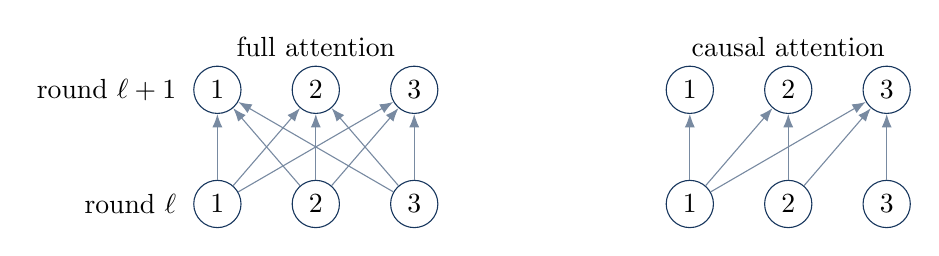
\begin{tikzpicture}[
  pnode/.style={circle,draw=courseblue,minimum size=6mm,inner sep=0pt},
  arr/.style={-{Latex[length=1.7mm]},courseblue!58,thin}]
  \begin{scope}
    \foreach \i in {1,2,3} {
      \node[pnode] (fx\i) at (1.25*\i,0) {$\i$};
      \node[pnode] (fh\i) at (1.25*\i,1.45) {$\i$};
    }
    \foreach \i in {1,2,3} {
      \foreach \j in {1,2,3} {\draw[arr] (fx\j)--(fh\i);}
    }
    \node at (2.5,2.0) {full attention};
  \end{scope}
  \begin{scope}[xshift=6.0cm]
    \foreach \i in {1,2,3} {
      \node[pnode] (cx\i) at (1.25*\i,0) {$\i$};
      \node[pnode] (ch\i) at (1.25*\i,1.45) {$\i$};
    }
    \draw[arr] (cx1)--(ch1);
    \draw[arr] (cx1)--(ch2); \draw[arr] (cx2)--(ch2);
    \draw[arr] (cx1)--(ch3); \draw[arr] (cx2)--(ch3);
    \draw[arr] (cx3)--(ch3);
    \node at (2.5,2.0) {causal attention};
  \end{scope}
  \node[anchor=east] at (.85,0) {round $\ell$};
  \node[anchor=east] at (.85,1.45) {round $\ell+1$};
\end{tikzpicture}
\caption{Every dependency allowed by full and causal attention on three
positions. A hard lookup selects one of the permitted sources for each
destination; the diagrams display the maximum set of possible arrows.}
\label{fig:attention-dependencies}
\end{figure}

\begin{lemma}[Prefix dependence]
\label{prop:prefix-causality}
In a program composed of causal selectors and positionwise maps, the state at
position $r$ after any number of rounds depends only on the input prefix
$(x_1,\ldots,x_r)$.
\end{lemma}

\begin{proof}
Use induction over rounds. The round-zero state at position $r$ uses only
$x_r$ and fixed positional information. A causal selector at position $r$
reads round-$\ell$ states only at positions $j\leq r$, which depend by the
induction hypothesis only on prefixes contained in $(x_1,\ldots,x_r)$; a
positionwise map adds no cross-position dependence.
\end{proof}

The lemma converts the causal mask into a reusable limitation on every later
state. In particular, a proposed parallel update is invalid if some position
must read a map record located later in the sequence. The causal analysis of
pointer doubling will use exactly this test.

\subsection{Associative lookup}

Associative lookup asks whether one fixed operation can use facts supplied in
the current sequence. The task is the basic operation behind dictionary
access: a query supplies a key and the sequence supplies the key--value
pairs. In a language context, the pairs may encode an attribute attached to a
name or a value assigned to a variable. Changing the names or adding more
pairs should not require new network parameters.

Let $\cD=\{k_1,\ldots,k_M\}$ be a set of distinct keys, let $\cV$ be an
arbitrary value set, and let $f:\cD\to\cV$. Store one pair at each of the
first $M$ sequence positions and place a query last:
\begin{equation}
 X(f,x)=\bigl((k_1,f(k_1)),\ldots,(k_M,f(k_M)),
 (\mathtt{QUERY},x)\bigr),
 \qquad x\in\cD.
 \label{eq:lookup-prompt}
\end{equation}
Associative lookup returns $f(x)$. The keys are symbols, not position
indices, and the values need not be keys.

One hard lookup round suffices. The final position uses $x$ as its query,
selects the unique earlier position whose key equals $x$, and retrieves the
value stored there. Equality matching and value retrieval do not depend on
$M$, so the same program handles every sequence length.

\begin{figure}[ht]
\centering
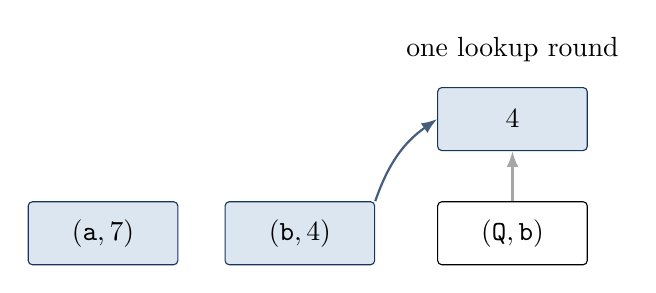
\begin{tikzpicture}[
  rec/.style={draw=courseblue,fill=lightblue,rounded corners=1.5pt,
    minimum width=19mm,minimum height=8mm},
  query/.style={draw,rounded corners=1.5pt,minimum width=19mm,
    minimum height=8mm},
  arr/.style={-{Latex[length=2mm]},thick,courseblue!80}]
  \node[rec] (a) at (0,0) {$({\mathtt a},7)$};
  \node[rec] (b) at (2.5,0) {$({\mathtt b},4)$};
  \node[query] (q) at (5.2,0) {$(\mathtt Q,{\mathtt b})$};
  \node[rec] (out) at (5.2,1.45) {$4$};
  \draw[arr] (b.north east) to[bend left=18] (out.west);
  \draw[-{Latex[length=2mm]},thick,gray!70] (q)--(out);
  \node[above=2mm of out] {one lookup round};
\end{tikzpicture}
\caption{Associative lookup with one key--value pair stored at each position.
The query matches the key $\mathtt b$ and retrieves the paired value $4$; the
gray arrow denotes the residual query state.}
\label{fig:associative-lookup}
\end{figure}

\begin{proposition}[Exact associative lookup]
\label{prop:associative-lookup}
Under the distinct-key and present-query assumptions, one hard attention
round computes $X(f,x)\mapsto f(x)$ for every finite key set $\cD$ and every
map $f:\cD\to\cV$. The construction is causal when the query follows all
stored pairs.
\end{proposition}

\begin{proof}
Distinctness and the assumption $x\in\cD$ give a unique index $r$ with
$k_r=x$. Equality matching therefore selects position $r$ and retrieves
$f(k_r)=f(x)$. The selected position precedes the query position, so the
lookup is causal. Neither the equality predicate nor the retrieval rule
depends on $M$.
\end{proof}

The one-pair-per-position encoding isolates the lookup operation from record
assembly. An ordinary token sequence may instead place the key and value at
consecutive positions,
\[
 (k_1,f(k_1),\ldots,k_M,f(k_M),\mathtt{QUERY},x).
\]
One preparation round lets every value position retrieve its predecessor key
and combine the retrieved key with its residual value. The resulting
key--value pairs support associative lookup in the next round.
\Cref{ex:l14-causal-lookup} asks you to compose two tables supplied
in the same input, so that the first retrieved value becomes the key for a
second lookup.

\subsection{Iterated lookup}
\label{sec:iterated-lookup}

A single lookup retrieves one supplied fact. Many symbolic computations use
the retrieved value to determine the next operation. For example, after
retrieving the mother of a person, the retrieved name becomes the key in the query for the
maternal grandmother. The second query is not known until the first lookup
has returned the selected value. Iterated lookup isolates the compositional
dependence.

Iteration becomes defined when the values are also keys. Specialize the same
formalism to a self-map $p:\cD\to\cD$ and ask for
\[
 p^K(x)=\underbrace{p\circ\cdots\circ p}_{K\ \text{copies}}(x),
 \qquad p^0(x)=x.
\]
The map is supplied by the pairs in $X(p,x)$; the network parameters specify
the lookup procedure, not the particular map.

The example in \cref{fig:sequential-lookup} uses exactly three lookups, so the
input needs only the three records on the queried path: Dana's mother, Cleo's
mother, and Bea's mother. Ada is the final returned value and need not appear
as a key. The general self-map formulation is needed only when every returned
value may become the key for another lookup. The same formal computation
models following links in a linked list, redirects in a table, or ancestors
in a rooted forest.

A direct procedure keeps the current key at the query position:
\begin{equation}
 z_0=x,
 \qquad z_{t+1}=p(z_t),
 \qquad t=0,\ldots,K-1.
 \label{eq:sequential-lookup}
\end{equation}
Round $t+1$ selects the pair keyed by $z_t$ and retrieves its value. Therefore
$z_t=p^t(x)$ by induction, and $K$ lookup rounds return $p^K(x)$. The
construction is causal for every self-map $p$ when all map pairs precede the
query.

\begin{figure}[ht]
\centering
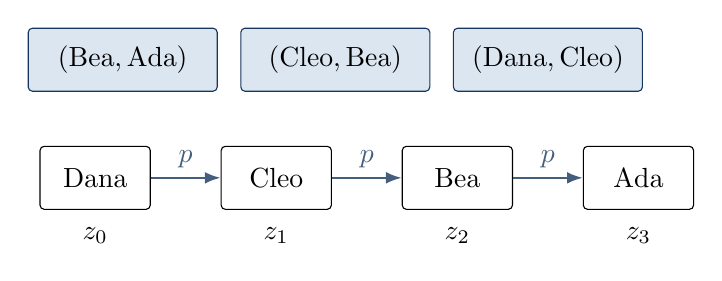
\begin{tikzpicture}[
  rec/.style={draw=courseblue,fill=lightblue,rounded corners=1.5pt,
    minimum width=24mm,minimum height=8mm},
  state/.style={draw,rounded corners=1.5pt,minimum width=14mm,
    minimum height=8mm},
  arr/.style={-{Latex[length=2mm]},thick,courseblue!80}]
  \node[rec] at (1.35,1.5) {$(\mathrm{Bea},\mathrm{Ada})$};
  \node[rec] at (4.05,1.5) {$(\mathrm{Cleo},\mathrm{Bea})$};
  \node[rec] at (6.75,1.5) {$(\mathrm{Dana},\mathrm{Cleo})$};
  \node[state] (z0) at (1.0,0) {Dana};
  \node[state] (z1) at (3.3,0) {Cleo};
  \node[state] (z2) at (5.6,0) {Bea};
  \node[state] (z3) at (7.9,0) {Ada};
  \draw[arr] (z0)--node[above] {$p$} (z1);
  \draw[arr] (z1)--node[above] {$p$} (z2);
  \draw[arr] (z2)--node[above] {$p$} (z3);
  \node[below=1mm of z0] {$z_0$};
  \node[below=1mm of z1] {$z_1$};
  \node[below=1mm of z2] {$z_2$};
  \node[below=1mm of z3] {$z_3$};
\end{tikzpicture}
\caption{A map described by the input and the successive query states. Each
arrow is one lookup round. With $p(u)$ equal to the mother of $u$, the states
name Dana, her mother, her maternal grandmother, and her maternal
great-grandmother.}
\label{fig:sequential-lookup}
\end{figure}

\subsection{Parallel pointer doubling}
\label{sec:pointer}

Transformers update all sequence positions in parallel. The direct procedure
above uses only the query position to advance along the map, so it takes $K$
sequential layers for $K$ map applications and leaves the parallel work at the
map-record positions unused. We now ask whether simultaneous computation at
those positions can return the same iterate in fewer sequential rounds.

Pointer doubling gives an affirmative answer under full attention. The map
positions preprocess the input map in parallel and store progressively longer
jumps. The construction reduces sequential depth by performing more parallel
work; it does not reduce the total number of table updates. The preprocessing
is especially useful when the same input map will answer many ancestor, link,
or redirect queries.
At the position keyed by $u\in\cD$, store
\begin{equation}
 q_0(u)=p(u),
 \qquad q_{\ell+1}(u)=q_\ell(q_\ell(u)).
 \label{eq:pointer-doubling}
\end{equation}
To perform one update, position $u$ uses its current value $q_\ell(u)$ as a
query key and retrieves $q_\ell(q_\ell(u))$ from the matching map position.
Every position performs the update simultaneously.

\begin{proposition}[Doubling invariant]
\label{prop:doubling}
For every self-map $p:\cD\to\cD$, every $u\in\cD$, and every $\ell\geq0$,
\[
 q_\ell(u)=p^{2^\ell}(u).
\]
Thus $L$ parallel doubling rounds transform the one-step table $q_0$ into the
$2^L$-step table $q_L$.
\end{proposition}

\begin{proof}
The base case is $q_0(u)=p(u)=p^{2^0}(u)$. If the invariant holds at round
$\ell$, then
\[
 q_{\ell+1}(u)
 =q_\ell(q_\ell(u))
 =p^{2^\ell}\bigl(p^{2^\ell}(u)\bigr)
 =p^{2^{\ell+1}}(u).
\]
Induction proves the invariant.
\end{proof}

The invariant contains two separate facts. First, all table entries can be
updated in parallel. Second, the resulting entries answer later queries: when
$K=2^L$, the query for $p^K(x)$ retrieves $q_L(x)$. For general $K$, retain
the fields $q_0,\ldots,q_{\lfloor\log_2 K\rfloor}$ and compose the fields
selected by the binary expansion of $K$. For example,
\[
 K=13=8+4+1,
 \qquad
 x\xrightarrow{q_3}p^8(x)
  \xrightarrow{q_2}p^{12}(x)
  \xrightarrow{q_0}p^{13}(x).
\]
The preprocessing and query phases each use $O(\log K)$ rounds.

\begin{figure}[ht]
\centering
\begin{tabular}{c@{\qquad}ccccc}
\toprule
key $u$ & $a$ & $b$ & $c$ & $d$ & $e$\\
\midrule
$q_0(u)=p(u)$ & $b$ & $c$ & $d$ & $e$ & $c$\\
$q_1(u)=p^2(u)$ & $c$ & $d$ & $e$ & $c$ & $d$\\
$q_2(u)=p^4(u)$ & $e$ & $c$ & $d$ & $e$ & $c$\\
\bottomrule
\end{tabular}
\vspace{2mm}

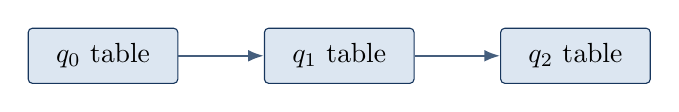
\begin{tikzpicture}[
  box/.style={draw=courseblue,fill=lightblue,rounded corners=1.5pt,
    minimum width=19mm,minimum height=7mm},
  arr/.style={-{Latex[length=2mm]},thick,courseblue!80}]
  \node[box] (r0) at (0,0) {$q_0$ table};
  \node[box] (r1) at (3.0,0) {$q_1$ table};
  \node[box] (r2) at (6.0,0) {$q_2$ table};
  \draw[arr] (r0)--(r1);
  \draw[arr] (r1)--(r2);
\end{tikzpicture}
\caption{Pointer doubling for the map
$a\mapsto b\mapsto c\mapsto d\mapsto e\mapsto c$. Each row is a stream
distributed across all five map positions. One round updates every column,
so two rounds produce the four-step map $q_2=p^4$.}
\label{fig:pointer-doubling}
\end{figure}

\subsection{What changes under causal attention}

Decoder-only transformers normally use a causal mask, so a full-attention
speedup is relevant only after checking that every retrieval respects the
sequence order. The sequential query construction in
\cref{eq:sequential-lookup} remains
causal for an arbitrary self-map: every map pair precedes the final query.
Parallel doubling imposes an additional requirement because a map position
must retrieve from another map position. Fix an order of the pairs and write
$\operatorname{pos}(u)$ for the position storing the pair keyed by $u$. The
first doubling update is causal when
\begin{equation}
 \operatorname{pos}(p(u))\leq\operatorname{pos}(u)
 \qquad\text{for every }u\in\cD.
 \label{eq:causal-map-order}
\end{equation}
The same inequality then holds for every iterate of $p$, so all later
doubling rounds are causal as well.

Condition~\eqref{eq:causal-map-order} is a restriction, not a relabeling that
works for every self-map. A family forest can be ordered with each mother
before her children. A directed cycle of length greater than one
cannot be ordered so that every edge points backward. In the special case
$\cD=[M]$ with the pair keyed by $i$ stored at position $i$, the condition is
$p(i)\leq i$; the graph points $(i,p(i))$ then lie on or below the diagonal
$y=x$. The picture resembles a discrete cobweb diagram, but the inequality is
needed only for causal parallel preprocessing, not for defining or computing
the iterates themselves.

\section{Extra reading: program correctness, representation, and learning}
\label{sec:claims}

The associative-lookup, iterated-lookup, and pointer-doubling constructions
prove the correctness of abstract lookup programs.
An empirical claim about a trained transformer requires two additional
steps: the architecture must implement the abstract operations with stated
resources, and training must find suitable parameters from finite data.
Keeping the three statements separate identifies what a construction, a
compiler theorem, or an experiment contributes:
\begin{enumerate}[leftmargin=*]
\item \textbf{Program correctness.} A symbolic sequence program computes the
desired map for every valid input.
\item \textbf{Model representation.} A specified transformer architecture
implements or approximates the program with stated depth, width, head count,
and numerical assumptions.
\item \textbf{Learning.} A specified training procedure, sample, and
optimization process produce parameters that execute the program, including
at lengths not used in training.
\end{enumerate}
The RASP language supports the first aspect by expressing streams, selectors,
and aggregations. Compiler results and direct constructions support the
second aspect for suitable transformer models. RASP-L restricts the program
language to operations intended to be length-uniform. The RASP-L
generalization claim is a conjecture supported by experiments: tasks with
short RASP-L programs tend to be learned with better length generalization.
Program existence alone does not imply that gradient-based training finds
the program.

RASP-L studies whether the existence of a short symbolic program predicts
length generalization across tasks. MicroPy examines a complementary
question: whether one learned transition mechanism can be applied many more
times at test time than occurred in training executions. A
59.5-million-parameter transformer was trained to execute programs whose
training traces contained at most 128 lines. Across
252 reported test instances, including bit operations, arithmetic, and SAT,
the model achieved 100 percent token accuracy; the longest successful
execution contained 7,552 trace lines, about 59 times the training cap. The
experiment demonstrates learned repeated computation in the trained MicroPy
system. The relevant extrapolation variable is execution-trace length; the reported
maximum test context was 2,197 tokens, and the paper does not give a matching
training-context range from which to infer context-length extrapolation.

\section{Extra reading: arithmetic assumptions}
\label{sec:arithmetic}

Counts of layers, heads, and coordinates do not by themselves specify the
computational resources of an exact construction. Equality tests may require
score margins, and a real-valued coordinate with unrestricted precision can
encode unbounded information.

The Boolean construction in \cref{sec:gates} uses small integer weights and
has exact semantics on bit inputs. The attention construction uses exact
equality predicates and hard selection. A finite-temperature softmax can
approximate a hard selector when the selected score has a positive margin,
but the required scale depends on that margin and the desired error.

Resource statements must therefore identify the arithmetic model. Fixed
finite precision bounds the number of distinguishable values in each internal
coordinate.
Growing precision introduces another resource. Unrestricted real parameters
can encode infinitely many bits and can hide advice about the answers. Size
and depth counts are meaningful when the construction also controls weight
magnitudes, margins, or bit complexity.

\section{Extra reading: a matching conditional lower bound}
\label{sec:lower-bound}

The pointer-doubling construction proves that logarithmic depth is sufficient.
A lower bound asks whether a substantially shallower parameter-efficient
masked transformer could solve the same kind of repeated-lookup problem by a
different method. There is a conditional lower bound for a standard repeated
lookup problem. For a sequence $X=(X_1,\ldots,X_N)$, define the previous-link
map
\[
 \operatorname{find}_X(i)
 =\max\bigl(\{0\}\cup\{j\in[N]:j\leq i,\ X_{j-1}=X_i\}\bigr),
\]
where position $0$ contains a distinguished null symbol. The $k$-hop task
iterates the previous-link map $k$ times and returns the symbol reached by the chain.

Assume the one-versus-two-cycle conjecture for massively parallel
computation. For any constants $\xi\in(0,1/2]$ and
$\varepsilon\in(0,1)$ and any even $k=\Theta(N^\xi)$, every masked
transformer that computes the $k$-hop task, has embedding dimension $m$, has
$H$ heads per layer, and satisfies
$mH=O(k^{1-\varepsilon})$ must have depth
\[
 L=\Omega(\log k).
\]
Sanford et al. also give an $O(\log k)$ masked-transformer construction for
the same task. The upper and lower bounds give a matching logarithmic
dependence on $k$ for parameter-efficient masked transformers, conditional on
the stated parallel-computation conjecture.

\section{Take-home messages}
\label{sec:take-home}

\begin{itemize}[leftmargin=*]
\item A Turing machine separates finite control from unbounded memory. Exact
representation of its finite transition table by a ReLU network, together
with repeated application and an external tape, is enough for universal
computation. The tape and repeated execution are required computational
resources.
\item Universal Boolean gates represent every Boolean function. ReLU networks
simulate a circuit of size $S$ and depth $D$ exactly with $O(S)$ size and
$O(D)$ depth. The proof compiles gates and uses induction over circuit layers.
\item Repeated composition can be exponentially more economical than one
hidden layer: $\tau^{\circ L}\in\cF_{L\text{-NN}}(3L)$, whereas
$\tau^{\circ L}\notin\cF_{1\text{-NN}}(2^L-2)$. The zero extension of the
tent map supplies a standard network map on $\R$; only its values on $[0,1]$
affect the iterates.
\item One length-uniform attention program can apply a map supplied as
key--value pairs in its input. If the stored values are also keys, $K$
successive rounds compose that supplied map and compute $p^K(x)$.
\item Under full attention, pointer doubling constructs the $2^L$-step map in
$L$ parallel rounds. Causal parallel doubling additionally requires the map
records to be ordered so that every retrieved record is no later than the
requesting record.
\item Program correctness, transformer representation, and learning the
program from data are distinct aspects. Exact constructions settle the first
two under stated models; RASP-L and MicroPy provide empirical evidence about
the third.
\end{itemize}

\printendnotes

\section*{Bibliographical notes}

The Church--Turing thesis is associated with the equivalent formalisms
introduced by \citet{church1936} and \citet{turing1937}. The lecture uses the
ordinary computability thesis, not the stronger claim that every physically
realizable process admits an efficient digital simulation.

\citet{newell1976} stated the physical symbol system hypothesis as a necessary
and sufficient account of general intelligent action. \citet{harnad1990}
formulated the symbol grounding problem and discussed learned nonsymbolic
representations as a possible component of grounding. Together, the physical
symbol system hypothesis and the grounding problem separate symbolic
representation from the question of how a system acquires its representations.

\citet{siegelmann1995} proved that a fixed finite recurrent neural network with
rational weights can simulate Turing computation under their synchronous
recurrent model. The elementary construction in
\cref{cor:neural-turing-control} instead places the unbounded tape explicitly
in the environment and uses the network only for finite control. Both results
show why representability and learnability must be analyzed separately.

The circuit-counting exercise uses the description-counting method of
\citet{shannon1949}: count the functions represented by circuits below a
given size and compare that count with the number of all Boolean functions.
The final lower bound is a pigeonhole argument and is nonconstructive.
The monotone and affine invariants in another exercise are elementary cases
of the composition-closed classes in \citet{post1941}.

The recurrent-automaton exercise isolates the finite-state part of the
simulation question. The fixed-precision exercise gives an elementary
finite-state limitation adjacent to the arithmetic assumptions in
\citet{perez2021}; their transformer completeness theorem instead permits
rational activations of arbitrary precision.

The tent-map construction and the use of rapidly growing oscillation to
separate deep and shallow networks follow the depth-separation program of
\citet{telgarsky2016}. The elementary one-dimensional breakpoint argument in
\cref{prop:shallow-pieces} is sufficient for the exact separation used here.
Telgarsky uses the term triangle function for the same single-peak shape.
The dynamical-systems interpretation of the tent map is developed by
\citet{alligood1997}; the period-three theorem is due to \citet{li1975}.

\citet{weiss2021} introduced RASP as a computational model for describing
transformer operations through sequence-valued maps, selection, and
aggregation. The language makes dependency and resource accounting visible.
\citet{zhou2024} introduced RASP-L and formulated the empirical conjecture
connecting short length-uniform programs with length generalization.

The associative-memory exercise uses the continuous Hopfield energy and
update studied by \citet{ramsauer2021}, whose update coincides with softmax
attention when the stored keys are also the retrieved values. The two-round
successor-retrieval exercise formalizes the induction-head mechanism studied
empirically by \citet{olsson2022}; the exercise proves only the stated abstract
lookup construction.

Pointer jumping is a classical parallel algorithm. The masked-transformer
$k$-hop construction and the conditional lower bound in
\cref{sec:lower-bound} are due to \citet{sanford2024}. Their paper also gives
unconditional tradeoffs for several restricted recurrent, kernel, and
sparse-attention architectures. The conditional result quoted here directly
matches logarithmic masked-transformer depth under the theorem's parameter
constraint.

The MicroPy experiment is reported by \citet{xu2026}. Its execution traces
externalize intermediate program state, allowing the same learned transition
mechanism to be applied many more times at test time than during training.

\section*{Glossary}

\begin{description}[style=unboxed,leftmargin=1.5em,labelindent=0pt]
\item[Physical symbol system hypothesis]
The hypothesis that a physical system capable of storing and manipulating
well-formed symbolic expressions by explicit rules has the necessary and
sufficient means for general intelligent action.
\item[Symbol grounding problem]
The problem of explaining how formal symbols become connected to objects,
properties, and situations outside the formal system, rather than receiving
the symbol-to-world connections only from an external interpretation.
\item[Turing-machine transition function]
The finite map from the current control state and scanned tape symbol to the
next state, written symbol, and head movement. The unbounded tape is separate
from the finite transition controller.
\item[Boolean circuit]
A directed acyclic graph of Boolean gates. Size counts gates; depth counts
the longest input-to-output gate path.
\item[Functionally complete gate set]
A collection of Boolean gates from which circuits can compute every Boolean
function on every finite number of inputs.
\item[Exact representation]
Equality between the target function and the network output on the stated
input domain, rather than approximation within a nonzero error tolerance.
\item[Affine piece]
A maximal interval on which a scalar function has the form $x\mapsto ax+b$.
\item[$\cF_{L\text{-NN}}(m)$]
The class of scalar functions represented by a ReLU network with $L$ hidden
layers and at most $m$ hidden ReLU units in total.
\item[Stream]
A sequence-valued variable $s:[N]\to\cD$ with one value per position.
\item[Causal selector]
A content- or position-dependent rule that lets position $i$ select only
positions $j\leq i$.
\item[Associative lookup]
Retrieval of the value paired with a specified key.
\item[Iterated lookup]
Repeated associative lookup for a self-map $p:\cD\to\cD$, where each returned
value supplies the key for the next lookup.
\item[Pointer doubling]
The parallel update $q_{\ell+1}(u)=q_\ell(q_\ell(u))$, which doubles the
number of original map applications represented after each stage.
\item[Length-uniform program]
One sequence program whose operations do not change with the input length.
\end{description}

\section{Exercises}
\label{sec:exercises}

\exerciseinstructions
\setcounter{courseexercise}{0}
\exercisegroup{Symbols and grounding}
\begin{exercisechunk}
\item \textbf{Symbol renaming and external grounding.}
\label[exercise]{ex:l14-symbol-renaming}
\exerciseprofile{2}{2}{2}{\exproof\quad\exinterpretation}{%
Separate invariance under symbol renaming from the external relation that
assigns meanings to symbols.}
This exercise gives a precise model of formal symbol manipulation. The model
isolates what equality, copying, and lookup preserve, and the final parts state
exactly what additional information a grounding relation supplies.

Let \(\cS\) be a finite set of symbols. A \emph{symbolic input} \(x\) is an
ordered finite collection of symbols together with zero or more finite tables
of ordered pairs from \(\cS\times\cS\). A deterministic \emph{symbolic
program} \(\cA\) has symbol registers and Boolean registers, contains no
hard-coded element of \(\cS\), and may perform only the following operations:
\begin{enumerate}[label=(\roman*),leftmargin=*]
\item copy a symbol from an input location or symbol register;
\item test whether two symbol registers contain the same symbol;
\item use a symbol as a key in an input table with distinct keys and copy the
corresponding value; and
\item branch according to a Boolean register.
\end{enumerate}
Assume that \(\cA\) terminates and returns one symbol in \(\cS\) on every
valid input.

Let \(\pi:\cS\to\cS\) be a bijection. Define \(\pi x\) by replacing every
symbol \(s\) occurring in \(x\), including every table key and value, by
\(\pi(s)\), while preserving positions and table order. For an output symbol
\(s\), the expression \(\pi(s)\) has its ordinary meaning: apply the map
\(\pi\) to \(s\). The program \(\cA\) itself is unchanged.
\begin{enumerate}[(a),beginpenalty=10000]
\item Prove that copying, equality testing, and table lookup commute with the
renaming \(\pi\). State the corresponding relation for each operation.
\item Prove by induction over the executed operations that
\[
 \cA(\pi x)=\pi\bigl(\cA(x)\bigr)
 \qquad\text{for every valid symbolic input }x.
\]
\item Let \(\cS=\{s_0,s_1\}\) and let
\(\cO=\{o_0,o_1\}\) be a set of external objects. A \emph{grounding} is a
bijection \(g:\cS\to\cO\). Consider
\[
 g_0(s_i)=o_i,
 \qquad
 g_1(s_i)=o_{1-i},
 \qquad i\in\{0,1\}.
\]
Fix one symbolic input \(x\), and suppose \(\cA\) receives neither \(g_0\)
nor \(g_1\). Prove that \(\cA(x)\) cannot name the target object \(o_0\)
under both groundings; that is, at least one of
\[
 g_0(\cA(x))=o_0,
 \qquad
 g_1(\cA(x))=o_0
\]
must fail.
\item Explain how parts~(b) and (c) differ. Your explanation must identify
what the renaming result proves, why the impossibility in part~(c) requires
the grounding to be absent from the input, and what kind of additional input
could break the ambiguity.
\end{enumerate}
\end{exercisechunk}

\exercisegroup{Boolean circuits and recurrent computation}
\begin{exercisechunk}
\item \textbf{Prove that unary gates cannot combine input bits.}
\label[exercise]{ex:l14-boolean-circuit}
\exerciseprofile{2}{2}{2}{\exproof\quad\exinterpretation}{%
Identify the structural limitation of circuits whose gates have at most one
input.}
Let $r\geq2$. Consider a Boolean circuit with input bits
$x_1,\ldots,x_r$ in which every gate has fan-in at most one. A zero-input
gate may output a constant, and a one-input gate may apply any function
$g:\{0,1\}\to\{0,1\}$. Fan-out is unrestricted.
\begin{enumerate}[(a),beginpenalty=10000]
\item Prove by induction over a topological ordering of the circuit that the
value at every gate is either constant or a function of one input coordinate
$x_i$.
\item Deduce that no such circuit computes
$\operatorname{AND}(x_1,x_2)$ or
$\operatorname{XOR}(x_1,x_2)$ on all four Boolean inputs.
\item List all four functions $g:\{0,1\}\to\{0,1\}$. Explain why allowing
every unary Boolean gate still does not give a functionally complete gate set
for functions of two or more input bits.
\end{enumerate}
\end{exercisechunk}

\begin{exercisechunk}
\item \textbf{Invariants that prevent functional completeness.}
\label[exercise]{ex:l14-boolean-invariants}
\exerciseprofile{2}{2}{2}{\exproof\quad\exinterpretation}{%
Use closure under composition to prove that two natural Boolean gate families
are not functionally complete.}
Functional completeness can fail because every available gate preserves a
property that some target Boolean function violates. This exercise develops
the monotone and affine invariants, two basic examples of that method.

For \(x,y\in\{0,1\}^r\), write \(x\le y\) when \(x_i\le y_i\) for every
\(i\). A Boolean function \(f\) is \emph{monotone} when
\(x\le y\) implies \(f(x)\le f(y)\). A Boolean function is \emph{affine over
\(\mathbb F_2\)} when it has the form
\[
 f(x)=c\oplus a_1x_1\oplus\cdots\oplus a_rx_r,
 \qquad c,a_1,\ldots,a_r\in\{0,1\},
\]
where \(\oplus\) denotes addition modulo two.
\begin{enumerate}[(a),beginpenalty=10000]
\item Prove that every circuit whose gates are monotone computes a monotone
function. Deduce that \(\{\operatorname{AND},\operatorname{OR},0,1\}\) is
not functionally complete.
\item Prove that composing affine Boolean functions produces another affine
Boolean function. Deduce that
\(\{\operatorname{XOR},\operatorname{NOT},0,1\}\) is not functionally
complete by proving that \(\operatorname{AND}\) is not affine.
\item State the general obstruction illustrated by parts~(a)--(b). Explain why
finding a composition-closed property shared by all available gates and
violated by one Boolean function is sufficient to disprove functional
completeness.
\end{enumerate}
\end{exercisechunk}

\begin{exercisechunk}
\item \textbf{Parity requires exponentially many DNF terms.}\suppmark
\label[exercise]{ex:l14-parity-dnf}
\exerciseprofile{2}{1}{2}{\exproof\quad\exconstruction\quad\exinterpretation}{%
Prove that changing the allowed representation can change parity from a
linear-size computation to an exponential-size formula.}
The parity function has a linear-size XOR circuit. This exercise proves that
the same function has no comparably small disjunctive normal form, so the
representation language is part of every size comparison.

Fix an integer \(r\geq 1\), and let
\[
 \operatorname{PARITY}_r(x)
 =x_1\oplus\cdots\oplus x_r,
 \qquad x\in\{0,1\}^r.
\]
A \emph{term} is a conjunction of literals, where a literal is \(x_i\) or
\(\operatorname{NOT}(x_i)\). A \emph{DNF} is a disjunction of terms. Terms
containing both \(x_i\) and \(\operatorname{NOT}(x_i)\) may be removed because
they are never satisfied.
\begin{enumerate}[(a),beginpenalty=10000]
\item Prove that exactly \(2^{r-1}\) inputs have parity one.
\item Let a satisfiable term occur in a DNF that computes
\(\operatorname{PARITY}_r\). Prove that the term must contain a literal for
every input coordinate. Deduce that the term is satisfied by at most one
input.
\item Prove that every DNF for \(\operatorname{PARITY}_r\) has at least
\(2^{r-1}\) terms. Construct a DNF with exactly \(2^{r-1}\) terms, and
therefore prove that the minimum number of terms is exactly \(2^{r-1}\).
\item Explain why the lower bound concerns the DNF representation and does not
contradict the existence of a linear-size XOR circuit.
\end{enumerate}
\end{exercisechunk}

\begin{exercisechunk}
\item \textbf{Most Boolean functions require large circuits.}
\label[exercise]{ex:l14-circuit-counting}
\exerciseprofile{2}{2}{2}{\exproof\quad\excalculation\quad\exinterpretation}{%
Use a counting argument to distinguish universal representation from efficient
representation.}
The Boolean universality theorem constructs a circuit for every Boolean
function, but the theorem does not give a small circuit for every function.
This exercise supplies the counting plan, so the task is to carry out its
consequences rather than invent a circuit encoding.

Fix \(r\) input bits. A circuit has \(s\) numbered gates in topological order.
Each gate chooses one of the sixteen functions
\(\{0,1\}^2\to\{0,1\}\), and each of its two ordered incoming wires may
come from an input or an earlier gate. The circuit output may be any input or
gate value. Let \(N_{r,s}\) be the number of Boolean functions representable
by circuits with at most \(s\) gates.
\begin{enumerate}[(a),beginpenalty=10000]
\item Prove the description-count bound
\[
 N_{r,s}
 \le (s+1)(r+s)\bigl(16(r+s)^2\bigr)^s.
\]
The bound may count several descriptions of the same circuit or function.
Explain why such overcounting does not invalidate the inequality.
\item Define
\[
 s_r=\left\lfloor\frac{2^r}{16r}\right\rfloor.
\]
Show that, for all sufficiently large \(r\),
\[
 \log_2 N_{r,s_r}
 \le 2r+3rs_r
 \le 2r+\frac{3}{16}2^r
 <2^r.
\]
You may use \(r+s_r\le2^r\) and \(4+2r\le3r\) once \(r\) is sufficiently
large.
\item There are \(2^{2^r}\) Boolean functions on \(r\) input bits. Deduce
that some Boolean function requires more than \(s_r\) gates. Show further
that the fraction of Boolean functions representable with at most \(s_r\)
gates tends to zero as \(r\to\infty\).
\item State what the argument establishes about circuit size and what it does
not provide about an explicit hard Boolean function.
\end{enumerate}
\begin{hints}
For part~(a), count descriptions gate by gate, using \(r+s\) as an upper
bound on every predecessor choice, and then choose the output. For part~(b),
take base-two logarithms before substituting \(s_r\). Part~(c) is a
pigeonhole argument.
\end{hints}
\end{exercisechunk}

\begin{exercisechunk}
\item \textbf{One ReLU unit cannot compute OR.}
\label[exercise]{ex:l14-or-single-relu}
\exerciseprofile{2}{1}{1}{\exproof\quad\excalculation\quad\exinterpretation}{%
Prove that one affine map followed by one ReLU cannot represent OR on the
Boolean domain.}
Let $g(x,y)=\operatorname{ReLU}(ax+by+c)$, where $a,b,c\in\R$.
Prove that no choice of $a,b,c$ makes $g(x,y)$ equal to
$\operatorname{OR}(x,y)$ for all $(x,y)\in\{0,1\}^2$.
\end{exercisechunk}

\begin{exercisechunk}
\item \textbf{Construct a recurrent ReLU simulation of a finite automaton.}
\label[exercise]{ex:l14-recurrent-dfa}
\exerciseprofile{2}{2}{2}{\exproof\quad\exconstruction\quad\exinterpretation}{%
Construct one fixed neural transition cell and distinguish its parameter count
from the number of times it is executed.}
The Turing-machine model separates finite control from external memory.
This exercise constructs the finite-control part directly and shows how
recurrence reuses one transition network for every input position.

Let \(Q\) and \(\Sigma\) be finite sets, and let
\(\delta:Q\times\Sigma\to Q\) be the transition function of a deterministic
finite automaton. Encode \(q\in Q\) and \(a\in\Sigma\) by the one-hot vectors
\(e_q\in\{0,1\}^{|Q|}\) and
\(e_a\in\{0,1\}^{|\Sigma|}\).
\begin{enumerate}[(a),beginpenalty=10000]
\item Construct a one-hidden-layer ReLU network
\[
 F:\R^{|Q|+|\Sigma|}\to\R^{|Q|}
\]
with at most \(|Q||\Sigma|\) hidden units and an affine output layer such
that
\[
 F(e_q,e_a)=e_{\delta(q,a)}
 \qquad(q\in Q,\ a\in\Sigma).
\]
Give all hidden-unit and output formulas.
\item For an input string \(a_1\cdots a_T\), define
\[
 h_0=e_{q_0},
 \qquad
 h_t=F(h_{t-1},e_{a_t}),\qquad t\in[T].
\]
Prove that \(h_t\) is the one-hot encoding of the automaton state after
reading \(a_1\cdots a_t\).
\item Compare the recurrent implementation with a feedforward network obtained
by unrolling \(T\) copies of \(F\). State separately how the number of distinct
parameters, the number of executed cell evaluations, and the unrolled depth
depend on \(T\).
\end{enumerate}
\begin{hints}
On bit inputs, one ReLU can indicate that two specified coordinates are both
one. If a second hint is needed, introduce one hidden unit for every pair
\((q,a)\in Q\times\Sigma\), then collect the pairs that lead to the same next
state.
\end{hints}
\end{exercisechunk}

\begin{exercisechunk}
\item \textbf{Finite precision produces an eventually periodic state.}\suppmark
\label[exercise]{ex:l14-finite-precision}
\exerciseprofile{2}{1}{2}{\exproof\quad\exinterpretation}{%
Identify the finite-state limitation created by fixed memory and fixed
precision.}
Turing-completeness claims depend on the available memory or numerical
precision. This exercise proves a limitation that follows from fixed finite
precision without using any architecture-specific lower bound.

Consider a deterministic recurrent system with \(d\) state coordinates, each
stored with exactly \(b\) bits. The system reads the unary input
\(a^t=a\cdots a\) one symbol at a time and produces one output bit after each
update. The state-update rule and output rule are fixed for all input lengths.
\begin{enumerate}[(a),beginpenalty=10000]
\item Prove that the recurrent system has at most \(2^{bd}\) internal states.
Deduce that its state sequence on the infinite unary stream
\(a,a,a,\ldots\) is eventually periodic, with both the preperiod and period
bounded by \(2^{bd}\).
\item Deduce that the output sequence is eventually periodic.
\item Let
\[
 \cL_{\mathrm{pow2}}=\{a^{2^k}:k\ge0\}.
\]
Prove that the indicator sequence
\(y_t=\I(a^t\in\cL_{\mathrm{pow2}})\) is not eventually periodic. Conclude
that no recurrent system satisfying the stated fixed-precision assumptions
recognizes \(\cL_{\mathrm{pow2}}\) correctly at every input length.
\item Explain which step of the proof fails when the system has an external
unbounded tape or a state coordinate whose available precision can grow with
the execution length.
\end{enumerate}
\end{exercisechunk}

\exercisegroup{Depth and symbolic dynamics}
\begin{exercisechunk}
\item \textbf{Construct the exact shallow form of an iterated tent map.}
\label[exercise]{ex:l14-tent-composition}
\exerciseprofile{2}{2}{2}{\exproof\quad\excalculation\quad\exconstruction\quad\exinterpretation}{%
Use slope changes to construct the smallest one-hidden-layer representation
allowed by the affine-skip form.}
Define the tent map on $[0,1]$ by
\[
 \tau(x)=\min\{2x,2-2x\}.
\]
Fix an integer $L\geq1$. You may use the lecture result that
$\tau^{\circ L}$ is affine on the $2^L$ dyadic subintervals of $[0,1]$ and
maps each subinterval onto $[0,1]$.
\begin{enumerate}[(a),beginpenalty=10000]
\item Show that the slope of $\tau^{\circ L}$ on the interval
$[j/2^L,(j+1)/2^L]$ is $(-1)^j2^L$. Use the slope changes at the interior
dyadic points to derive
\[
 \tau^{\circ L}(x)
 =2^Lx+2^{L+1}\sum_{j=1}^{2^L-1}(-1)^j
 \operatorname{ReLU}\left(x-\frac{j}{2^L}\right),
 \qquad x\in[0,1].
\]
\item Consider the one-hidden-layer form
\[
 f(x)=a_0+a_1x+
 \sum_{r=1}^m c_r\operatorname{ReLU}(w_rx+b_r).
\]
Use part~(a) and the lecture's breakpoint lower bound to prove that the
smallest $m$ for which this form can equal $\tau^{\circ L}$ on $[0,1]$ is
exactly $2^L-1$.
\item Compare the shallow representation from part~(b) with the membership
$\tau^{\circ L}\in\cF_{L\text{-NN}}(3L)$. State separately how depth and
the total number of hidden units scale with $L$ in the two constructions.
\end{enumerate}
\end{exercisechunk}

\begin{exercisechunk}
\item \textbf{A robust separation from alternating tent-map labels.}
\label[exercise]{ex:l14-tent-robust-separation}
\exerciseprofile{3}{2}{3}{\exproof\quad\excalculation\quad\exinterpretation}{%
Extend the exact folding separation to a quantitative classification-error
lower bound.}
The lecture proves that an exact shallow representation of an iterated tent
map needs exponentially many hinges. This exercise shows that a shallow
network also needs exponentially many pieces to obtain small error on a
specified finite classification problem.

Fix \(L\ge1\), put \(N=2^L\), and define
\[
 x_j=\frac{j+1/4}{N},
 \qquad
 y_j=\I\bigl(\tau^{\circ L}(x_j)\ge1/2\bigr),
 \qquad j=0,\ldots,N-1.
\]
For a scalar function \(f\), define
\[
 \widehat y_j(f)=\I(f(x_j)\ge1/2),
 \qquad
 \operatorname{err}_L(f)
 =\frac1N\sum_{j=0}^{N-1}\I\bigl(\widehat y_j(f)\ne y_j\bigr).
\]
\begin{enumerate}[(a),beginpenalty=10000]
\item Use the slopes and endpoint values of \(\tau^{\circ L}\) to prove
\[
 \tau^{\circ L}(x_j)
 =\begin{cases}1/4,&j\text{ even},\\[1mm]3/4,&j\text{ odd},\end{cases}
 \qquad
 y_j=j\bmod2.
\]
\item Let \(\widehat y_0,\ldots,\widehat y_{N-1}\) be any binary sequence
with \(R\) maximal constant runs. Prove that its number of disagreements with
the alternating sequence \(0,1,0,1,\ldots\) is at least \((N-R)/2\).
\item Suppose \(f\) is continuous and affine on at most \(K\) intervals.
Prove that \(\widehat y_0(f),\ldots,\widehat y_{N-1}(f)\) has at most \(2K\)
constant runs. Deduce
\[
 \operatorname{err}_L(f)
 \ge \frac12-\frac{K}{2^L}.
\]
\item A one-hidden-layer scalar ReLU network with \(m\) hidden units is affine
on at most \(m+1\) intervals. Prove that
\[
 \operatorname{err}_L(f)<\frac14
 \quad\Longrightarrow\quad
 m+1>2^{L-2}.
\]
Compare this necessary shallow width with the \(O(L)\)-unit deep
representation of \(\tau^{\circ L}\).
\end{enumerate}
\begin{hints}
For part~(b), count the errors inside each constant run separately. For
part~(c), the superlevel set of an affine function on one interval is empty,
the full interval, or an interval touching one endpoint.
\end{hints}
\end{exercisechunk}

\begin{exercisechunk}
\item \textbf{Symbolic histories of the tent map.}
\label[exercise]{ex:l14-tent-symbolic-dynamics}
\exerciseprofile{2}{2}{2}{\exproof\quad\excalculation\quad\exinterpretation}{%
Connect the affine pieces of an iterated tent map with uniformly distributed
binary symbolic histories.}
The term \emph{symbolic dynamics} records which branch of a dynamical system
an orbit visits. This exercise shows that the \(2^L\) affine pieces of the
tent-map iterate correspond exactly to \(L\)-bit branch histories.

Let \(X\) be uniformly distributed on \([0,1]\) under the ambient probability
measure \(\P\). Define
\[
 B_t=\I\bigl(\tau^{\circ t}(X)\ge1/2\bigr),
 \qquad t=0,1,\ldots.
\]
Events involving dyadic endpoints may be assigned to either adjacent branch;
these endpoints have probability zero.
\begin{enumerate}[(a),beginpenalty=10000]
\item Prove directly from the two inverse branches of \(\tau\) that
\[
 \P(\tau(X)\le y)=y,
 \qquad 0\le y\le1.
\]
Thus \(\tau(X)\) is uniformly distributed on \([0,1]\).
\item For \(b=(b_0,\ldots,b_{L-1})\in\{0,1\}^L\), define
\[
 C_b=\left\{x\in[0,1]:
 \I(\tau^{\circ t}(x)\ge1/2)=b_t
 \text{ for }t=0,\ldots,L-1\right\}.
\]
Prove by induction on \(L\) that, up to endpoints, \(C_b\) is one interval
of length \(2^{-L}\), and \(\tau^{\circ L}\) maps that interval affinely
onto \([0,1]\).
\item Deduce that
\[
 \P(B_0=b_0,\ldots,B_{L-1}=b_{L-1})=2^{-L}
 \qquad(b\in\{0,1\}^L).
\]
Conclude that \(B_0,\ldots,B_{L-1}\) are independent Bernoulli random
variables with success probability \(1/2\).
\item Use part~(a) inductively to identify the law of
\(\tau^{\circ t}(X)\) for every \(t\ge0\). Explain how parts~(b)--(c)
relate the \(2^L\) affine pieces to symbolic histories rather than merely
counting pieces.
\end{enumerate}
\end{exercisechunk}

\exercisegroup{Lookup, attention, and associative memory}
\begin{exercisechunk}
\item \textbf{Compose two input-specified lookup tables.}
\label[exercise]{ex:l14-causal-lookup}
\exerciseprofile{2}{2}{2}{\exproof\quad\excalculation\quad\exconstruction\quad\exinterpretation}{%
Use the output of one associative lookup as the query for a second table.}
Let
\[
 f:\{\mathtt a,\mathtt b\}\to\{1,2\},
 \qquad
 g:\{1,2\}\to\{\mathtt{red},\mathtt{blue}\}
\]
be specified by
\[
 f(\mathtt a)=2,\quad f(\mathtt b)=1,
 \qquad
 g(1)=\mathtt{red},\quad g(2)=\mathtt{blue}.
\]
The input sequence contains the tagged records
\[
 ((\mathtt F,\mathtt a,2),(\mathtt F,\mathtt b,1),
  (\mathtt G,1,\mathtt{red}),(\mathtt G,2,\mathtt{blue}),
  (\mathtt{QUERY},\mathtt b)).
\]
In one lookup round, the final position may form a query from its current
state, equality-select one earlier tagged record, retrieve that record's
value, and update its state. All lookups must be causal.
\begin{enumerate}[(a),beginpenalty=10000]
\item List the query, selected record, retrieved value, and updated final
state in each of two rounds that return $g(f(\mathtt b))$. Compute the final
answer.
\item Let $\cD,\cV,\cW$ be finite sets, let $f:\cD\to\cV$ and
$g:\cV\to\cW$, and suppose the input contains tagged records for both maps
followed by a query $x\in\cD$. Assume the keys in each table are distinct.
Give one two-round lookup program and prove that its output is $g(f(x))$ for
every choice of the two tables and every allowed set size.
\item Explain why the final query position cannot in general return
$g(f(x))$ in one round under the stated one-record-per-round abstraction.
Identify one change to the input representation that would make one-round
retrieval possible.
\end{enumerate}
\end{exercisechunk}

\begin{exercisechunk}
\item \textbf{Construct a two-round induction lookup.}
\label[exercise]{ex:l14-induction-head}
\exerciseprofile{2}{2}{2}{\exproof\quad\exconstruction\quad\exinterpretation}{%
Show how one attention round constructs predecessor--current records and a
second round uses those records for content-based retrieval.}
An induction head retrieves the token that followed an earlier occurrence of
the current token. The construction below expresses that mechanism as two
causal lookup rounds and makes the dependency between the rounds explicit.

Let \(x_1,\ldots,x_n\in\cS\), where \(n\ge3\). Assume that there is a unique
index \(j\in[n-2]\) such that \(x_j=x_n\), and that no other index in
\([n-1]\) contains \(x_n\). Initially, position \(i\) stores \(x_i\) and its
position index. A round may use a fixed positional query or an equality query,
retrieve one causal source state, and combine the retrieved value with the
destination's residual state.
\begin{enumerate}[(a),beginpenalty=10000]
\item Give a first causal round after which every position \(i\ge2\) stores
the record \((x_{i-1},x_i)\). State the source selected at position \(i\) and
the residual information retained there.
\item Give a second causal round at position \(n\) that uses \(x_n\) as a key
and returns \(x_{j+1}\). Identify the unique selected position.
\item Prove that the two-round program returns the token following the unique
earlier occurrence of \(x_n\) for every sequence satisfying the assumptions.
\item Explain why the required key--value record is absent from the round-zero
states. Under the stated one-source-per-round abstraction, identify the two
dependent retrievals that prevent the same construction from being performed
in one round.
\end{enumerate}
\end{exercisechunk}

\begin{exercisechunk}
\item \textbf{Attention as a modern Hopfield update.}\suppmark
\label[exercise]{ex:l14-hopfield-attention}
\exerciseprofile{2}{2}{2}{\exproof\quad\excalculation\quad\exinterpretation}{%
Derive the energy update underlying softmax attention and quantify its approach
to hard associative lookup.}
Earlier exercises analyze how score ranges control softmax concentration and
retrieval error. The new result here is the energy interpretation: when keys
are also values, one softmax-attention update is one gradient step for a
modern Hopfield energy.

Let \(M\ge2\), let \(k_1,\ldots,k_M\in\R^d\), let \(\beta>0\), and define
\[
 \alpha_i(q)=\frac{e^{\beta k_i^\top q}}
 {\sum_{j=1}^M e^{\beta k_j^\top q}},
 \qquad
 E_\beta(q)=\frac12\|q\|_2^2-
 \frac1\beta\log\left(\sum_{i=1}^M e^{\beta k_i^\top q}\right).
\]
\begin{enumerate}[(a),beginpenalty=10000]
\item Differentiate \(E_\beta\) and prove
\[
 \nabla E_\beta(q)=q-\sum_{i=1}^M\alpha_i(q)k_i.
\]
\item Show that one gradient step of length one gives
\[
 q^+=q-\nabla E_\beta(q)
 =\sum_{i=1}^M\alpha_i(q)k_i.
\]
Identify the queries, keys, and values in the corresponding one-query
attention operation. Explain why a general attention output
\(\sum_i\alpha_i(q)v_i\) with arbitrary \(v_i\) need not be a gradient step
in the query space \(\R^d\).
\item Suppose \(i^\star\) uniquely maximizes \(k_i^\top q\), define
\[
 \Delta=k_{i^\star}^\top q-\max_{i\ne i^\star}k_i^\top q>0,
\]
and assume \(\|k_i\|_2\le B\) for every \(i\). You may use
\[
 1-\alpha_{i^\star}(q)
 \le (M-1)e^{-\beta\Delta}.
\]
Prove
\[
 \|q^+-k_{i^\star}\|_2
 \le2B(M-1)e^{-\beta\Delta}.
\]
For \(0<\varepsilon<2B(M-1)\), give a sufficient lower bound on \(\beta\)
for this error to be at most \(\varepsilon\).
\item Explain which limit produces hard associative lookup and identify the
roles of the score margin \(\Delta\), the number of memories \(M\), and the
norm bound \(B\) in the quantitative approximation.
\end{enumerate}
\end{exercisechunk}

\pagebreak[3]
\begin{exercisechunk}
\item \textbf{When does a reusable jump table reduce the total cost?}\suppmark
\label[exercise]{ex:l14-pointer-doubling}
\exerciseprofile{2}{2}{2}{\exproof\quad\excalculation\quad\exinterpretation}{%
Count the preprocessing and query operations that the asymptotic depth
comparison suppresses.}
Let $p:\cD\to\cD$ be a self-map on a set of size $M$. Suppose full-attention
preprocessing has constructed
\[
 q_\ell(u)=p^{2^\ell}(u),
 \qquad \ell=0,\ldots,J,
\]
at every map-record position. Constructing each of
$q_1,\ldots,q_J$ costs $M$ table updates.
Count one application of a stored table entry to one key as one table lookup,
and count the construction of one new $q_\ell(u)$ value as one table update.
\begin{enumerate}[(a),beginpenalty=10000]
\item Let $K=\sum_{\ell=0}^J b_\ell2^\ell$, where
$b_\ell\in\{0,1\}$. Prove that applying the maps $q_\ell$ for which
$b_\ell=1$ returns $p^K(x)$ in any order. Deduce that the query uses
$\sum_{\ell=0}^J b_\ell$ lookups.
\item Consider the exhaustive batch containing one query for every
$K\in\{0,\ldots,2^{J+1}-1\}$. Compute exactly the total number of lookups
used by direct iteration and by the stored jump tables. Your answer should
include the $MJ$ preprocessing updates in the jump-table total.
\item Suppose instead that the same input map must answer $Q$ queries, each
with iteration count
$K_{\max}=2^{J+1}-1$ but possibly with a different initial state. Compute
the total jump-table cost and the total direct-iteration cost. State an
inequality on $M,Q,K_{\max}$ under which the jump tables use fewer total
operations.
\item Compare the exhaustive batch in part~(b) with the maximum-length batch
in part~(c). Explain why a sequential-depth advantage
does not by itself imply a reduction in the total number of table
operations.
\end{enumerate}
\end{exercisechunk}

\begin{exercisechunk}
\item \textbf{Characterize causally orderable self-maps.}\suppmark
\label[exercise]{ex:l14-causal-order}
\exerciseprofile{2}{2}{2}{\exproof\quad\exconstruction\quad\exinterpretation}{%
Characterize exactly when every pointer update can retrieve from an earlier
record in one causal ordering.}
The pointer-doubling construction requires an ordering in which every map
record points backward or to itself. This exercise identifies exactly which
finite self-maps admit such an ordering.

Let \(p:\cD\to\cD\) be a self-map on a finite set. Its functional directed
graph has one edge \(u\to p(u)\) from every vertex. A \emph{causal ordering}
is a bijection \(\operatorname{pos}:\cD\to[|\cD|]\) satisfying
\[
 \operatorname{pos}(p(u))\le\operatorname{pos}(u)
 \qquad(u\in\cD).
\]
\begin{enumerate}[(a),beginpenalty=10000]
\item Prove that if the functional graph contains a directed cycle of length
greater than one, then no causal ordering exists.
\item Suppose every directed cycle is a self-loop. Prove that every orbit
eventually reaches a unique fixed point in its connected component. Define the
depth of a vertex to be the number of map applications needed to reach that
fixed point. Construct a causal ordering and prove that it satisfies the
required inequality.
\item Conclude that a causal ordering exists if and only if every directed
cycle is a self-loop.
\item Prove that a causal ordering also satisfies
\[
 \operatorname{pos}(p^k(u))\le\operatorname{pos}(u)
 \qquad(u\in\cD,\ k\ge0).
\]
Explain why this inequality makes every lookup in causal pointer-doubling
preprocessing available at or before the requesting record.
\end{enumerate}
\end{exercisechunk}


\begin{thebibliography}{99}
\raggedright
\small

\bibitem[Alligood et al.(1997)]{alligood1997}
Kathleen T. Alligood, Tim D. Sauer, and James A. Yorke.
\newblock \emph{Chaos: An Introduction to Dynamical Systems}.
\newblock Springer, 1997.
\newblock \url{https://doi.org/10.1007/978-3-642-59281-2}.

\bibitem[Church(1936)]{church1936}
Alonzo Church.
\newblock An unsolvable problem of elementary number theory.
\newblock \emph{American Journal of Mathematics}, 58(2):345--363, 1936.
\newblock \url{https://doi.org/10.2307/2371045}.

\bibitem[Hajnal et al.(1993)]{hajnal1993}
Andr\'as Hajnal, Wolfgang Maass, Pavel Pudl\'ak, M\'ari\'o Szegedy, and
Gy\"orgy Tur\'an.
\newblock Threshold circuits of bounded depth.
\newblock \emph{Journal of Computer and System Sciences}, 46(2):129--154,
1993.
\newblock \url{https://doi.org/10.1016/0022-0000(93)90001-D}.

\bibitem[H\r{a}stad(1986)]{hastad1986}
Johan H\r{a}stad.
\newblock Almost optimal lower bounds for small depth circuits.
\newblock In \emph{Proceedings of the 18th Annual ACM Symposium on Theory of
Computing}, pages 6--20, 1986.
\newblock \url{https://doi.org/10.1145/12130.12132}.

\bibitem[H\r{a}stad et al.(2017)]{hastad2017}
Johan H\r{a}stad, Benjamin Rossman, Rocco A. Servedio, and Li-Yang Tan.
\newblock An average-case depth hierarchy theorem for Boolean circuits.
\newblock \emph{Journal of the ACM}, 64(5), article 35, 2017.
\newblock \url{https://doi.org/10.1145/3095799}.

\bibitem[Harnad(1990)]{harnad1990}
Stevan Harnad.
\newblock The symbol grounding problem.
\newblock \emph{Physica D: Nonlinear Phenomena}, 42(1--3):335--346, 1990.
\newblock \url{https://doi.org/10.1016/0167-2789(90)90087-6}.

\bibitem[Kane and Williams(2016)]{kane2016}
Daniel M. Kane and Ryan Williams.
\newblock Super-linear gate and super-quadratic wire lower bounds for
depth-two and depth-three threshold circuits.
\newblock In \emph{Proceedings of the 48th Annual ACM Symposium on Theory of
Computing}, pages 633--643, 2016.
\newblock \url{https://doi.org/10.1145/2897518.2897636}.

\bibitem[Krishnan and Mossel(2026)]{krishnan2026}
Neil Krishnan and Elchanan Mossel.
\newblock Depth lower bounds for ReLU networks with binary inputs.
\newblock arXiv:2606.18540, 2026.
\newblock \url{https://arxiv.org/abs/2606.18540}.

\bibitem[Li and Yorke(1975)]{li1975}
Tien-Yien Li and James A. Yorke.
\newblock Period Three Implies Chaos.
\newblock \emph{American Mathematical Monthly}, 82(10):985--992, 1975.
\newblock \url{https://doi.org/10.1080/00029890.1975.11994008}.

\bibitem[Newell and Simon(1976)]{newell1976}
Allen Newell and Herbert A. Simon.
\newblock Computer science as empirical inquiry: Symbols and search.
\newblock \emph{Communications of the ACM}, 19(3):113--126, 1976.
\newblock \url{https://doi.org/10.1145/360018.360022}.

\bibitem[Olsson et al.(2022)]{olsson2022}
Catherine Olsson et al.
\newblock In-context learning and induction heads.
\newblock arXiv:2209.11895, 2022.
\newblock \url{https://arxiv.org/abs/2209.11895}.

\bibitem[P\'erez et al.(2021)]{perez2021}
Jorge P\'erez, Pablo Barcel\'o, and Javier Marinkovic.
\newblock Attention is Turing-complete.
\newblock \emph{Journal of Machine Learning Research}, 22(75):1--35, 2021.
\newblock \url{https://www.jmlr.org/papers/v22/20-302.html}.

\bibitem[Post(1941)]{post1941}
Emil L. Post.
\newblock \emph{The Two-Valued Iterative Systems of Mathematical Logic}.
\newblock Annals of Mathematics Studies 5. Princeton University Press, 1941.

\bibitem[Ramsauer et al.(2021)]{ramsauer2021}
Hubert Ramsauer et al.
\newblock Hopfield networks is all you need.
\newblock In \emph{International Conference on Learning Representations},
2021.
\newblock \url{https://openreview.net/forum?id=tL89RnzIiCd}.

\bibitem[Sanford et al.(2024)]{sanford2024}
Clayton Sanford, Daniel Hsu, and Matus Telgarsky.
\newblock Transformers, parallel computation, and logarithmic depth.
\newblock In \emph{Proceedings of the 41st International Conference on
Machine Learning}, volume 235 of \emph{Proceedings of Machine Learning
Research}, pages 43276--43327, 2024.
\newblock \url{https://proceedings.mlr.press/v235/sanford24a.html}.

\bibitem[Siegelmann and Sontag(1995)]{siegelmann1995}
Hava T. Siegelmann and Eduardo D. Sontag.
\newblock On the computational power of neural nets.
\newblock \emph{Journal of Computer and System Sciences}, 50(1):132--150,
1995.
\newblock \url{https://doi.org/10.1006/jcss.1995.1013}.

\bibitem[Shannon(1949)]{shannon1949}
Claude E. Shannon.
\newblock The synthesis of two-terminal switching circuits.
\newblock \emph{Bell System Technical Journal}, 28(1):59--98, 1949.
\newblock \url{https://doi.org/10.1002/j.1538-7305.1949.tb03624.x}.

\bibitem[Telgarsky(2016)]{telgarsky2016}
Matus Telgarsky.
\newblock Benefits of depth in neural networks.
\newblock In \emph{Proceedings of the 29th Conference on Learning Theory},
volume 49 of \emph{Proceedings of Machine Learning Research}, pages
1517--1539, 2016.
\newblock \url{https://proceedings.mlr.press/v49/telgarsky16.html}.

\bibitem[Turing(1937)]{turing1937}
Alan M. Turing.
\newblock On computable numbers, with an application to the
Entscheidungsproblem.
\newblock \emph{Proceedings of the London Mathematical Society},
s2-42(1):230--265, 1937.
\newblock \url{https://doi.org/10.1112/plms/s2-42.1.230}.

\bibitem[Weiss et al.(2021)]{weiss2021}
Gail Weiss, Yoav Goldberg, and Eran Yahav.
\newblock Thinking like transformers.
\newblock In \emph{Proceedings of the 38th International Conference on
Machine Learning}, volume 139 of \emph{Proceedings of Machine Learning
Research}, pages 11080--11090, 2021.
\newblock \url{https://proceedings.mlr.press/v139/weiss21a.html}.

\bibitem[Xu et al.(2026)]{xu2026}
Ruize Xu, Chenxiao Yang, Yanhong Li, and David McAllester.
\newblock Training transformers as a universal computer.
\newblock arXiv:2604.25166, 2026.
\newblock \url{https://arxiv.org/abs/2604.25166}.

\bibitem[Zhou et al.(2024)]{zhou2024}
Hattie Zhou, Arwen Bradley, Etai Littwin, Noam Razin, Omid Saremi,
Josh Susskind, Samy Bengio, and Preetum Nakkiran.
\newblock What algorithms can transformers learn? A study in length
generalization.
\newblock In \emph{The Twelfth International Conference on Learning
Representations}, 2024.
\newblock \url{https://proceedings.iclr.cc/paper_files/paper/2024/hash/45ed1a72597594c097152ef9cc187762-Abstract-Conference.html}.

\end{thebibliography}

\end{document}
